\documentclass[journal,onecolumn]{IEEEtran}
\usepackage[pdftex]{graphicx}
\usepackage{epstopdf}
\epstopdfsetup{update}
\usepackage{amsmath, amssymb}
\usepackage{url}
\usepackage{float}
\usepackage{todonotes}
\usepackage{siunitx}
\usepackage{amsmath}
\usepackage{amssymb}
\usepackage{caption}
\usepackage{subcaption}
\usepackage{subfigure}

% correct bad hyphenation here
\hyphenation{op-tical net-works semi-conduc-tor}


\begin{document}

% VoMi uncomment this to learn the width of our page (for matlab to properly plot stuff)
%\showthe\textwidth % For single column documents
%\showthe\columnwidth % For multiple column documents

\title{BVM13TMO Semestral Work}
\author{Vojtěch Michal, michavo3}

% The paper headers
\markboth{BVM13TMO Semestral Work, Vojtěch Michal}%

% make the title area
\maketitle

% As a general rule, do not put math, special symbols or citations
% in the abstract or keywords.
\begin{abstract}
This report is a semestral work.
\end{abstract}

% Note that keywords are not normally used for peerreview papers.
\begin{IEEEkeywords}
Battery modelling, state estimation.
\end{IEEEkeywords}



\chapter{Week 2 -- BMS Temperature Stability}
\section{Abstract}
This report presents the results of measurements required by the assignment\footnote{accesiable via \url{https://moodle.fel.cvut.cz/pluginfile.php/474390/mod_resource/content/0/CV02_BMS.pdf}}. The laboratory task focuses on the temperature stability of the voltage threshold of three distinct cell balancing circuits. Their U-I characteristics were measured at various temperatures to assess the variability of voltage thresholds in real applications.


\section{Experimental setup}

\IEEEPARstart{T}{he} set of three cell balancing circuits -- devices under test -- with cell connection pads exposed as marked wires was enclosed into a box with a heating element and a thermometer. The voltage-current characteristics of individual devices were measured at several temperatures. Each measurement was performed manually using a programmable power supply used in the constant current operating mode. For each specified value of the discharging current, the corresponding voltage reading was recorded. This method suffered from inaccuracy by neglecting some factors, such as the wire resistance. Furthermore, the power supply only provides voltage readings with a resolution of 1 mV, which was insufficient to obtain more detailed U-I characteristics in the proximity of threshold voltage. Therefore the U-I characteristic is assumed to be piecewise linear in two regions
\begin{equation}
    i(u) = \begin{cases}
    0 & \text{if }  u < u_{\rm{T}}, \\
    \frac{u - u_{\rm{T}}}{R} & \text{if }  u \ge u_{\rm{T}},
    \end{cases}
\end{equation}
where $u_{\rm{T}}$ is the threshold voltage.

\section{Experimental results and conclusions}




\begin{figure}[htbp]
    \centering
    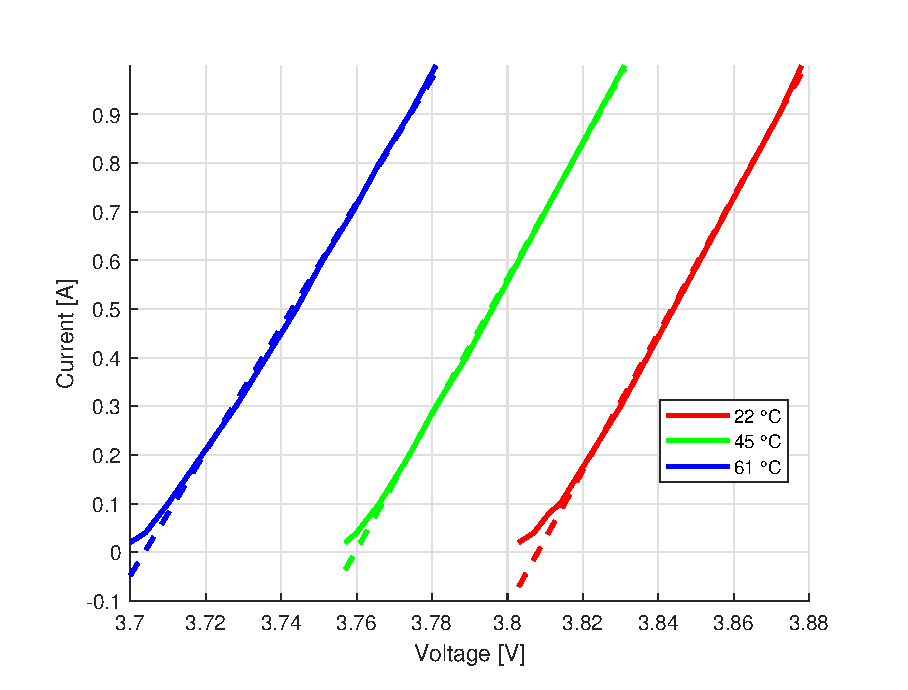
\includegraphics[width=0.5\linewidth]{figures/2/sample_A.eps}
    \caption{U-I characteristic of sample A}
    \label{fig:2-sample-A}
\end{figure}

Measured voltage-current characteristics of sample A for various temperatures are shown in Fig. \ref{fig:2-sample-A} together with their corresponding linear approximations. The threshold voltage is calculated as the x-intercept of the linear approximation. It is clear that the threshold voltage significantly varies with temperature approximately according to
\begin{equation}
    u_{\rm T} (\theta) \approx -0.0026~\theta + 3.8695 \text{ V},
\end{equation}
where $\theta$ is the temperature in °C.

Results for sample B are shown in Fig. \ref{fig:2-sample-B}, hinting that this sample is far more stable than sample B. The approximate temperature dependence of the threshold voltage is
\begin{equation}
    u_{\rm T} (\theta) \approx -0.0002~\theta + 3.9481 \text{ V},
\end{equation}
so more than an order of magnitude more stable.

\begin{figure}[htbp]
    \centering
    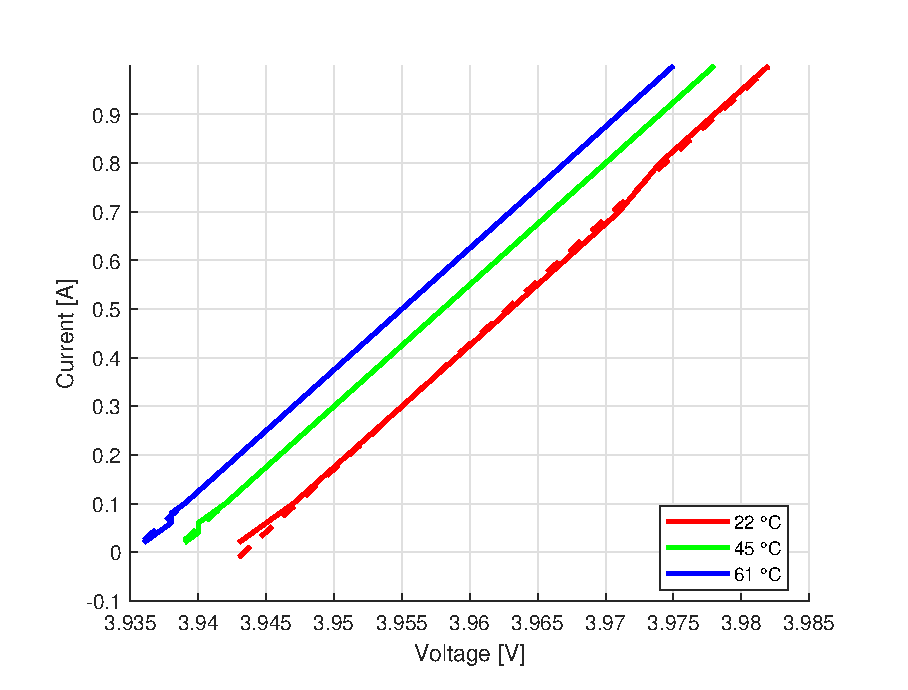
\includegraphics[width=0.5\linewidth]{figures/2/sample_B.eps}
    \caption{U-I characteristic of sample B}
    \label{fig:2-sample-B}
\end{figure}

No characteristics were measured for the sample C, as that BMS employed digital control via an integrated circuit, making it impossible to measure any static characteristic, as the discharge resistor was switched at irregular intervals according to the BMs internal logic.


\chapter{Week 3 -- MATLAB}

This report presents the results of tasks required by the assignment\footnote{accesiable via \vomihwassignment}. The exercise focused on the basics of the MATLAB environment and its utilization for processing of large datasets. As an illustration, the report demonstrated results from processing a dataset of several cell charge/discharge cycles.

\section{Abstract}

\section{Experimental results}

Table \ref{tab:3-dchg-cap} lists discharge capacities recorded during individual cycles.

\begin{table}[htbp]
    \centering
    \begin{tabular}{|c|c|c|c|c|c|c|}
    \hline
         cycle ID & 1 & 2 & 3 & 4 & 5 & 6 \\\hline
         Discharging capacity Q [Ah] &  3.163   &    3.1505       & 3.1311  &     3.1164   &    3.1049      & 3.2172 \\\hline
    \end{tabular}
    \caption{Discharging capacity available at each recorded cycle}
    \label{tab:3-dchg-cap}
\end{table}

\begin{figure}[htbp]
    \centering
    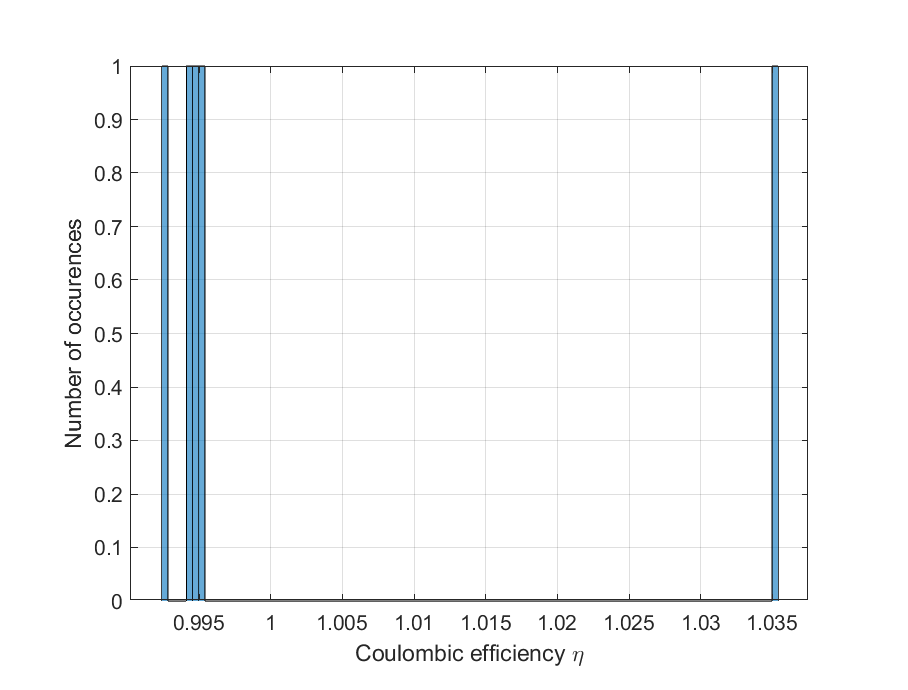
\includegraphics[width=0.75\linewidth]{figures/3/etas.eps}
    \caption{Histogram of coulombic efficiencies $\eta$ from completed cycles}
    \label{fig:3-etas}
\end{figure}

Histogram of coulombic efficiencies recorded for individual cycles is show in Fig. \ref{fig:3-etas}. It only shows data from complete cycles (i.e. without the first cycle). An interesting detail is the occurrence of number greater than one -- this $\eta$ corresponds to the last cycle, where a significantly lower current of 1 A (compared to previously used 3 A) was used to discharge the cell. Lower current lead to lower terminal voltage drop when loaded and therefore the cell was able to discharge more charge before the cycle ended safely. Otherwise the efficiency can't be higher than 1. The state of charge at each time during the experiment is shown in Fig. \ref{fig:3-soc}.


\begin{figure}[htbp]
    \centering
    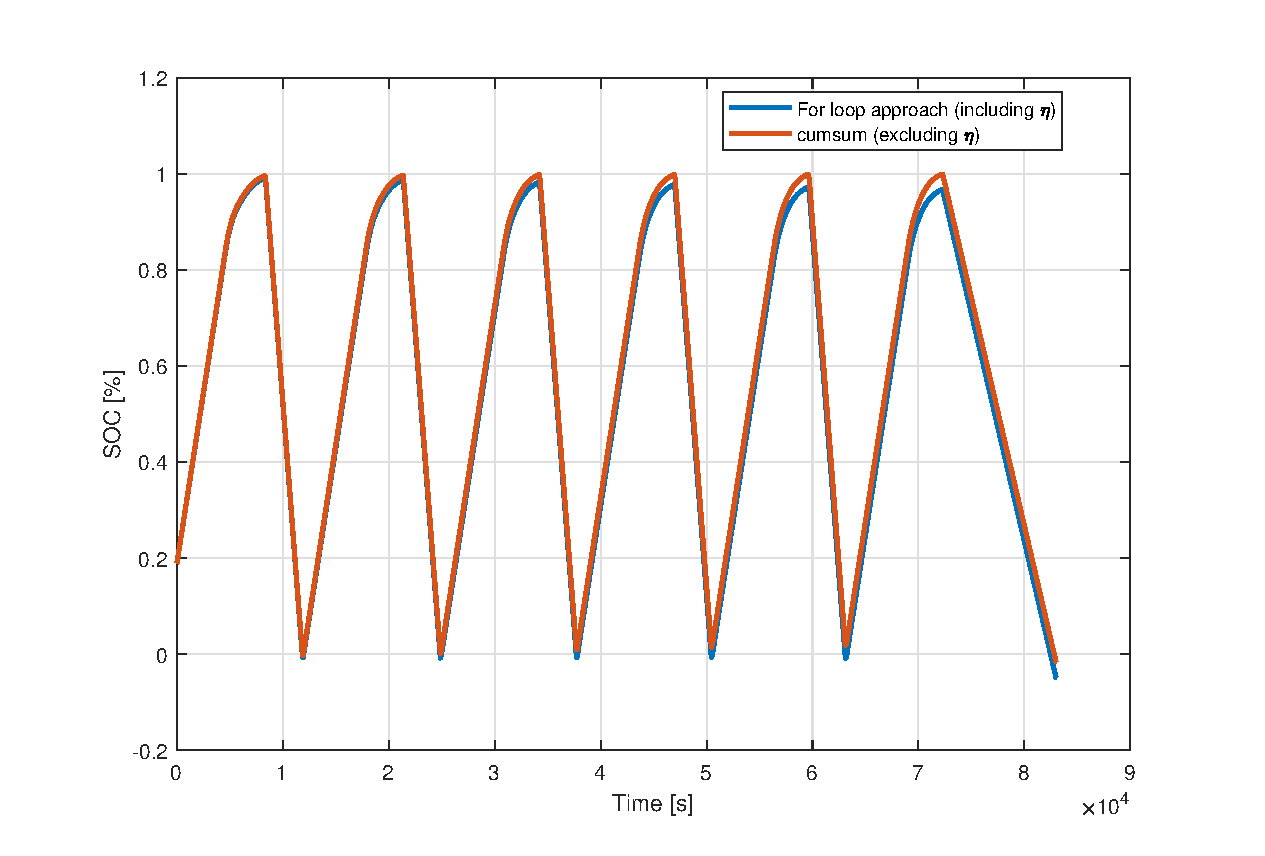
\includegraphics[width=0.75\linewidth]{figures/3/soc.eps}
    \caption{State of charge calculated using two different methods}
    \label{fig:3-soc}
\end{figure}

Cell data from the second charge-discharge cycle are shown in Fig. \ref{fig:3-tiled-layout}, clearly showing the CC-CV charging mode and the successive CC discharge.

\begin{figure}[htbp]
    \centering
    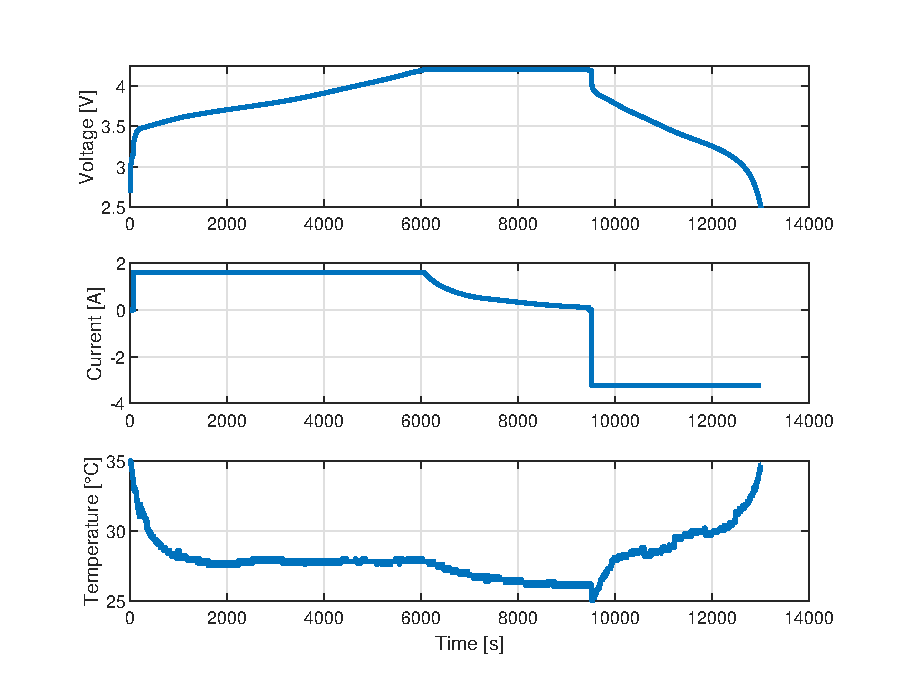
\includegraphics[width=0.75\linewidth]{figures/3/tiledlayout.eps}
    \caption{Voltage, current and temperature of cell during second charge-discharge cycle}
    \label{fig:3-tiled-layout}
\end{figure}



\begin{figure}[htbp]
    \centering
    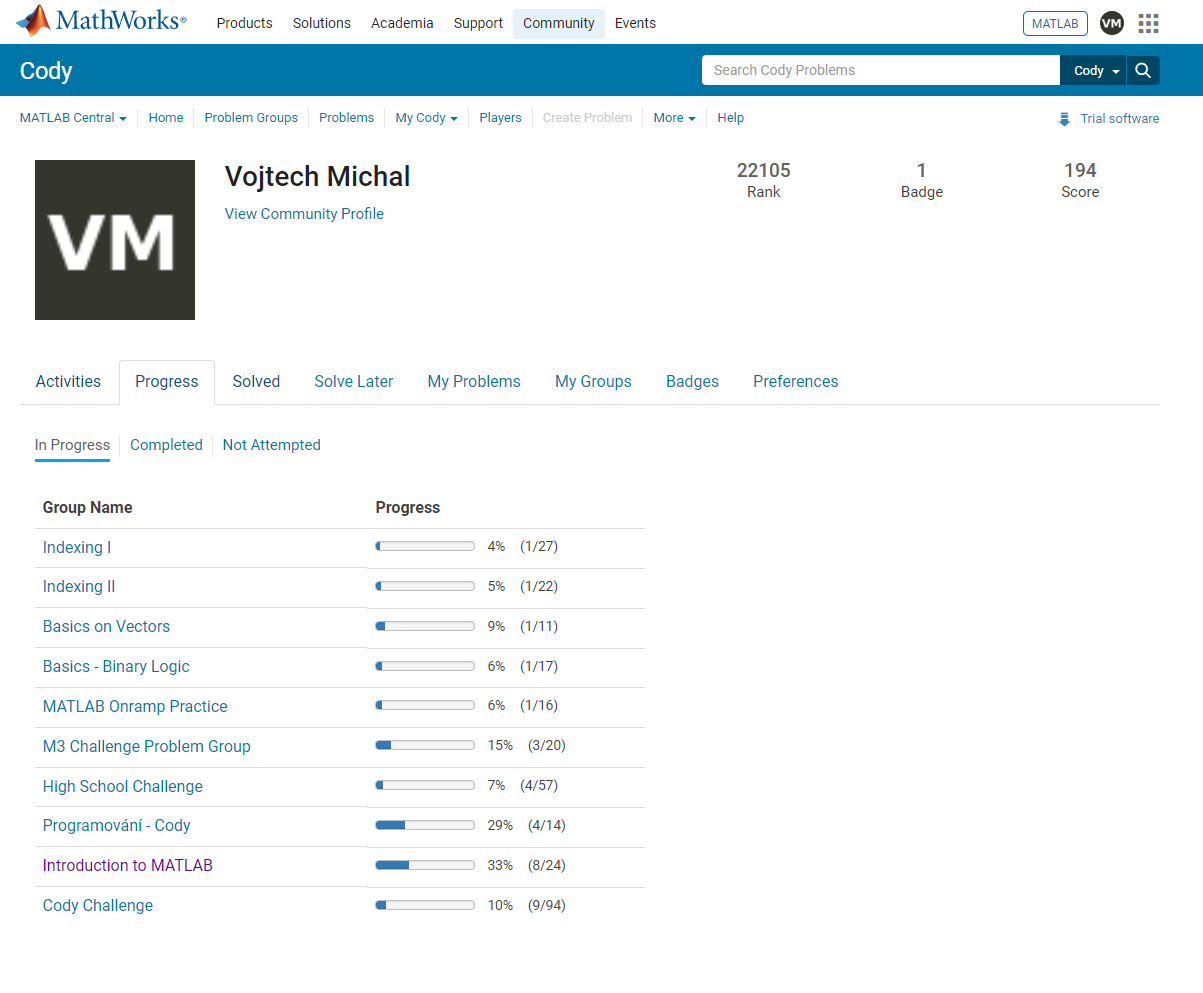
\includegraphics[width=0.99\linewidth]{figures/3/Cody.png}
    \caption{Proof of finished Matlab Cody exercises}
    \label{fig:3-cody}
\end{figure}

\chapter{Week 4 -- Battery testing}
% As a general rule, do not put math, special symbols or citations
% in the abstract or keywords.
\section{Abstract}
This report presents the results of simple battery testing procedure required by the assignment\footnote{accesiable via \vomihwassignment}. Constant current charging and discharging pulses were applied to the cell under test in order to estimate basic parameters of the equivalent circuit model using the measured voltages. This procedure was repeated twice, once "manually" using a programmable power supply and DC load and once by programming a dedicated battery tester.

\section{Charging pulse}

During the charging experiment, the cell was charged by a constant current of 1 A for 20 seconds. Afterwards the cell was allowed to rest for 5 minutes to restore open circuit voltage. Charging was performed using the 
laboratory power supply \textit{BK PRECISION 9205}. No dedicated voltage measurement was provided, instead
only readings from the instrument's display with resolution of 1 mV were recorded. Readings inherently contain
voltage drop across the leads as well. Furthermore it is impossible to correctly record fast transients when enabling/disabling the power supply.
This significantly reduced the reliability of equivalent circuit parameters $R_0$, $R_1$ and $C_1$ estimated in section \ref{sec:4-params}.
The voltage profile together with the applied current is shown in Fig. \ref{fig:4-charging}.

\begin{figure}[htbp]
    \centering
    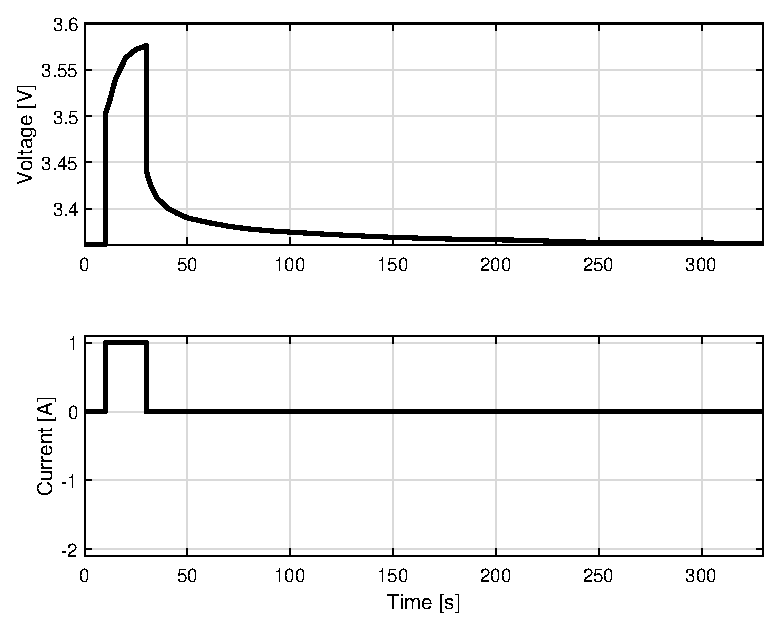
\includegraphics{figures/4/charge.eps}
    \caption{Voltage profile during the charging pulse experiment}
    \label{fig:4-charging}
\end{figure}

\section{Discharging pulse}
In this experiment, the cell was discharged by a constant current of 2 A for 20 seconds and allowed to rest for 5 minutes afterwards.
Discharging was performed using the DC programmable load \textit{BK PRECISION 8601}. Since no dedicated voltage measurement was provided, measurements from this experiment suffer from the same errors as discussed for the charging experiment. Measurements were recorded using the instrument's display with resolution of 0.1 mV.
The voltage profile together with the applied current is shown in Fig. \ref{fig:4-discharging}.


\begin{figure}[htbp]
    \centering
    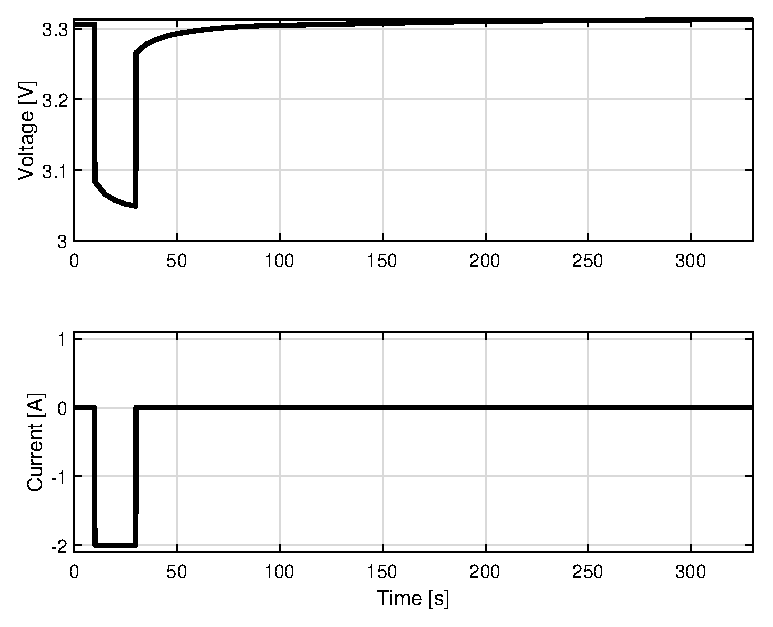
\includegraphics{figures/4/discharge.eps}
    \caption{Voltage profile during the discharging pulse experiment}
    \label{fig:4-discharging}
\end{figure}

\section{Automated experiment}
An automated battery tester \textit{Newell BT-4008Tn-5V12A-S1} was programmed to perform a complete experiment containing 20 seconds of (dis)charging interleaved by relaxation time. Since the instrument (and the experimental setup overall) is professional, it can be assumed that some lead resistance is compensated in the recorded data. The instrument was configured to save quantities with sampling period 100 ms to correctly record fast transients when applying new value of current. The voltage profile together with the applied current is shown in Fig. \ref{fig:4-automated}.

\begin{figure}[htbp]
    \centering
    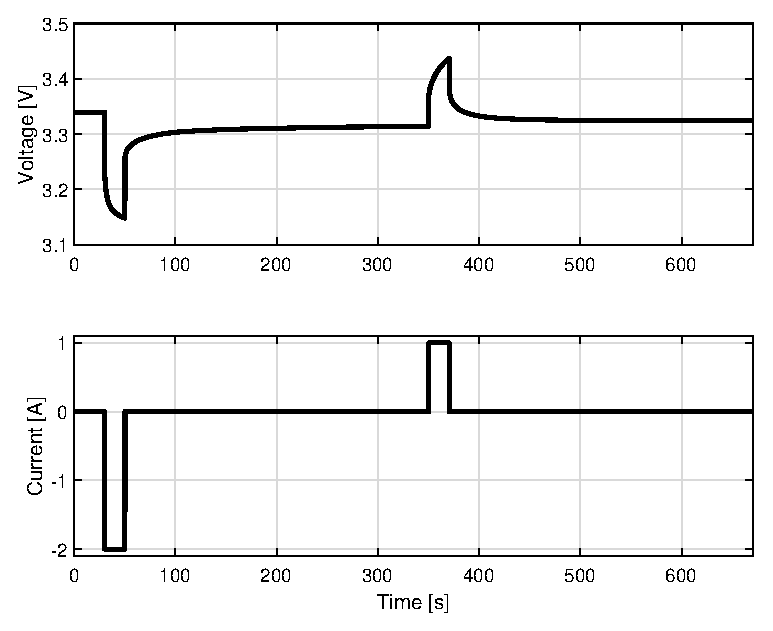
\includegraphics{figures/4/automated.eps}
    \caption{Voltage profile during the automated experiment}
    \label{fig:4-automated}
\end{figure}

\section{Parameter estimation}
\label{sec:4-params}
Data recorded during three experiments were used to estimate parameters of the equivalent circuit model with series impedance $R_0$ and one RC element $R_1$, $C_1$. Estimated values are shown in table \ref{tab:4-params}. It can be concluded that although the experimental setup for manual charging/discharging was very simple, it yielded reasonable estimates that are at least within the order of magnitude from the expected value. Automated measurements performed by the programmable battery tester are far more accurate. This manifests especially in the case of parameter $R_0$, whose value is almost equal for both automated discharge as well as charge experiment. It is not possible to give a certain estimate of $R_0$
for either of the manual experiments due to low refresh rate of instruments' displays. Recording a video of instrument's screen also isn't a particularly error resistant and high sampling rate method for data processing.

\begin{table}[htbp]
    \centering
    \begin{tabular}{c|c|c|c}
         Experiment& $R_0$ [$\Omega$] & $R_1$ [$\Omega$] & $C_1$ [F] \\\hline
         Manual discharge  & 1.116e-01  &   2.355e-02  &   2.547e+03 \\
         Manual charge & 1.410e-01   &  7.801e-02 &    7.6897e+02 \\
         Automated discharge & 5.664e-02  &   2.825e-02  &   2.124e+03 \\
         Automated charge & 5.701e-02   &  5.539e-02  &   1.083e+03
  
    \end{tabular}
    \caption{Estimated parameters of the cell model}
    \label{tab:4-params}
\end{table}


\chapter{Week 5 -- Implementation of Mathematical Models}

\section{Abstract}
This report presents the Matlab implementation of a dynamic battery model based on an equivalent circuit. A battery cell is first modelled as a voltage source with internal impedance. Subsequently, two RC elements in series with internal impedance are added. Temperature and SOC dependence of individual parameters is considered as well. The cell model was fully parameterized in the assignment. Equations governing the behaviour of the given model were implemented in Matlab code to facilitate simulation.


\section{Simple battery model}

The first implemented model considered only an ideal voltage source $U_{OC}$ with impedance $R_0$ in series. The only state is the state of charge (here given in percent rather than in the range $\left[0, 1\right]$. The flowing current $I$ is the model input and the voltage across battery terminals $U_{bat}$ is the only output. This model is is governed by the state space
\begin{equation}
\begin{split}
    \dot{SOC} &= -\eta \frac{1}{C} I, \\
    U_{bat} &= U_{OC} - I R_0.
\end{split}
\label{eq:5-simple}
\end{equation}

The model was simulated over a time interval of 500 seconds with results shown in Fig. \ref{fig:5-simple}. Since the battery has total capacity of 3 Ah and the discharging current averages to 1 A, simple calculation predicts decrease of SOC by roughly 4.6 \%. Since this prediction matches the simulation result, one can conclude that the simulation yields sane results.


\begin{figure}[hbtp]
    \centering
    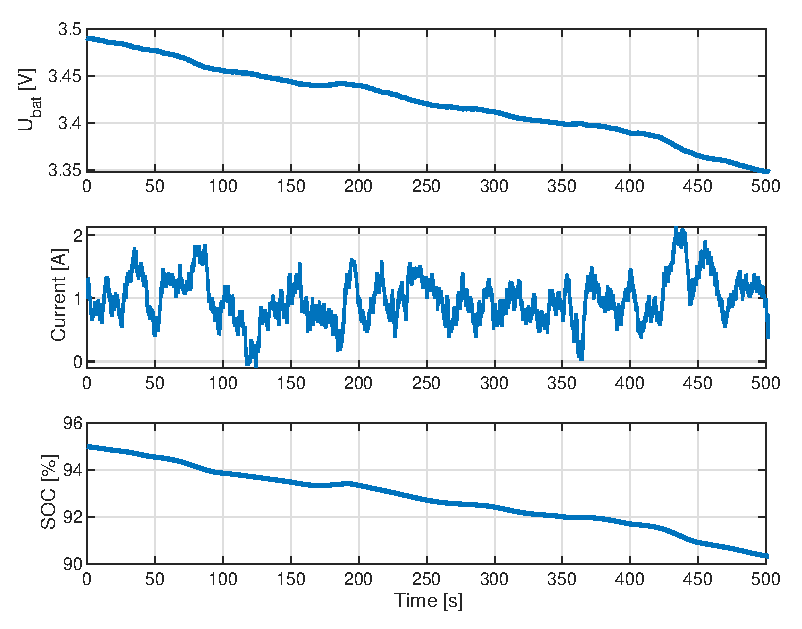
\includegraphics[width=0.8\textwidth]{figures/5/simple-everything.eps}
    \caption{Simulation results for simple battery model}
    \label{fig:5-simple}
\end{figure}

\section{Improved battery model}

The second implemented model added two RC elements with parameters $R_i$ and $C_i$ on top of the already considered simple model. This modification adds two states -- voltage drop $U_i$ across each RC element. This model is is governed by the state space
\begin{equation}
\begin{split}
    \dot{SOC} &= -\eta \frac{1}{C} I, \\
    \dot{U_1} &= -\frac{1}{R_1 C_1} U_1 + \frac{1}{C_1} I, \\
    \dot{U_2} &= -\frac{1}{R_2 C_2} U_2 + \frac{1}{C_2} I, \\
    \dot{SOC} &= -\eta \frac{1}{C} I, \\
    U_{bat} &= U_{OC} - I R_0 - U_1 - U_2.
\end{split}
\label{eq:5-complex}
\end{equation}


whose parameters are all temperature-dependent.

The model was simulated over a time interval of 500 seconds using temperature shown in Fig. \ref{fig:5-complex-temp} with results shown in Fig. \ref{fig:5-complex}. The discharged SOC again matches the expected value of roughly 5 \%. The terminal voltage $U_{bat}$ is generally lower than in case of the simple model since both models use identical values of the internal impedance $R_0$ and the improved model adds additional voltage drops. These observations prove the sanity of the implemented model and obtained results.

 Individual voltage drops across each RC element as well as the internal impedance $R_0$
 are shown in detail in Fig. \ref{fig:5-complex-RC}. Note how the voltage drop across $R_0$
 is negligible compared to the drop across each RC element -- $R_0$ is at least an order of magnitude lower than $R_1$ or $R_2$. This also explains why the terminal voltage $U_{bat}$ in Fig. \ref{fig:5-simple} is much smoother than $U_{bat}$ in Fig. \ref{fig:5-complex}.
 
\begin{figure}
    \centering
    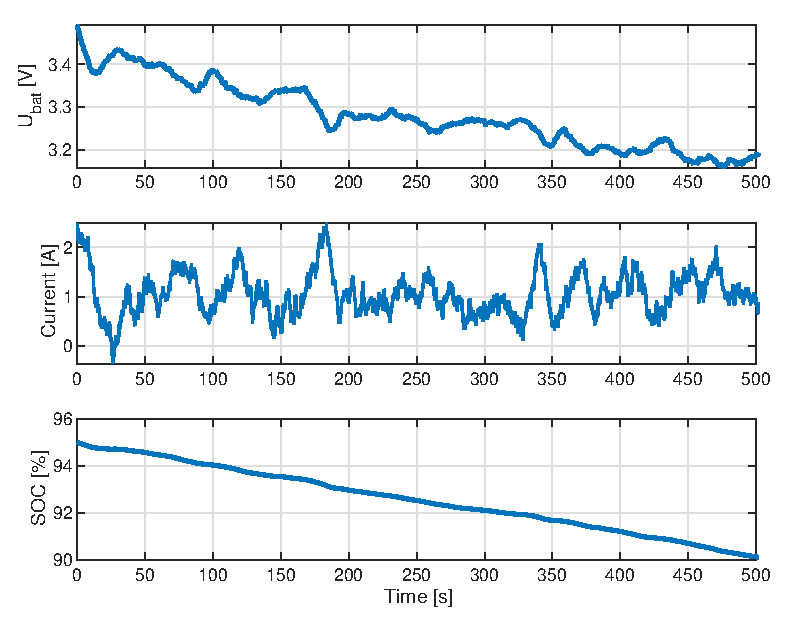
\includegraphics[width=0.8\textwidth]{figures/5/complex-everything.eps}
    \caption{Simulation results for improved battery model with two RC elements}
    \label{fig:5-complex}
\end{figure}

\begin{figure}
    \centering
    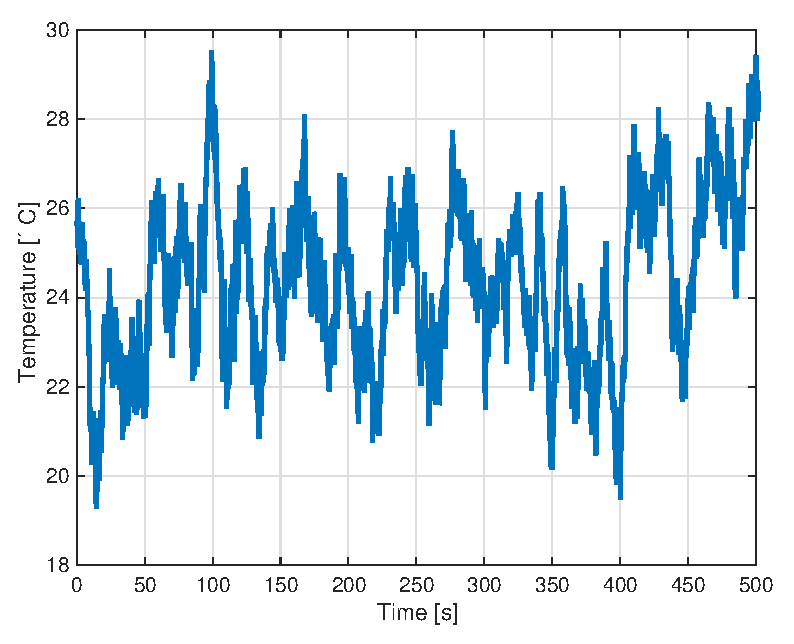
\includegraphics[width=0.6\textwidth]{figures/5/complex-Temp.eps}
    \caption{Temperature used for improved model simulation}
    \label{fig:5-complex-temp}
\end{figure}

\begin{figure}
    \centering
    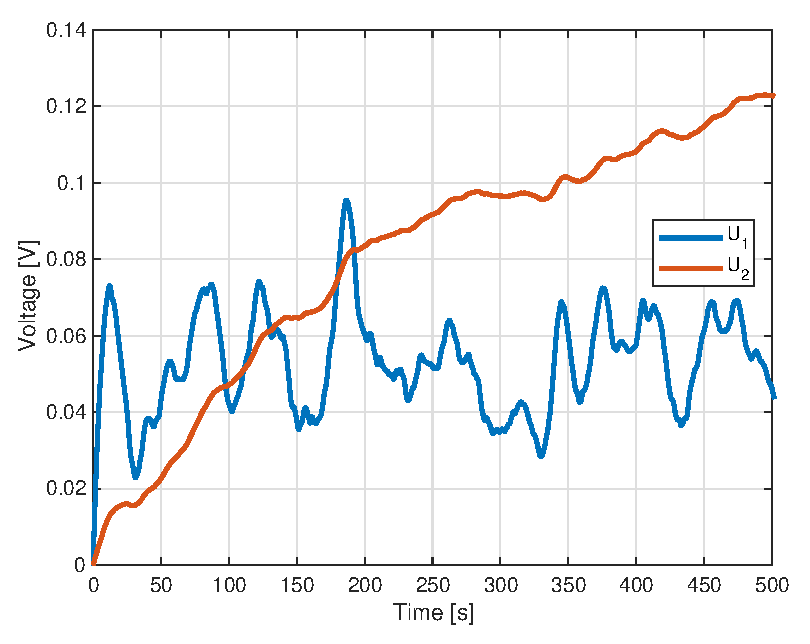
\includegraphics[width=0.6\textwidth]{figures/5/complex-U-RC.eps}
    \caption{Simulated voltage drops across each component of the improved model}
    \label{fig:5-complex-RC}
\end{figure}




\chapter{Parametrization and Validation of Battery Models}

\section{Abstract}
This report presents results of parametrization and subsequent validation of a battery model using measured experimental data. Experimental recordings of slow charge and discharge cycle are used to estimate the open-circuit voltage $U_\text{OC}$ as a function of SOC. A pulse test is used to identify equivalent circuit model parameters $R_0$, $R_1$ and $C_1$. All estimates are verified using a testing data set with dynamic discharge profile.


\section{Open circuit voltage test}

During the identification experiment, the cell went through a full charge-discharge cycle using a small current of 120 mA. First, I wanted to include identification of hysteresis (both maximal magnitude as well as its dynamics represented by the decay rate $\gamma$), but I have given up on this task due to the limited amount of available data. Although it would be possible to estimate the maximal magnitude of hysteresis by simply subtracting the charging and discharging voltage curve and compensating the voltage drop on internal resistance, this piece of information would be worthless. The training data set lacks any sufficiently dynamic experiment where the hysteresis decay rate could be reliably identified, hence I would have to tune it using the validation data, which is against the point of validation.

Hence only the OCV curve as a function of SOC was obtained by averaging the voltage curve from charge and discharge half-cycle. All relevant curves can be seen in Fig. \ref{fig:6-ocv}.

\begin{figure}
    \centering
    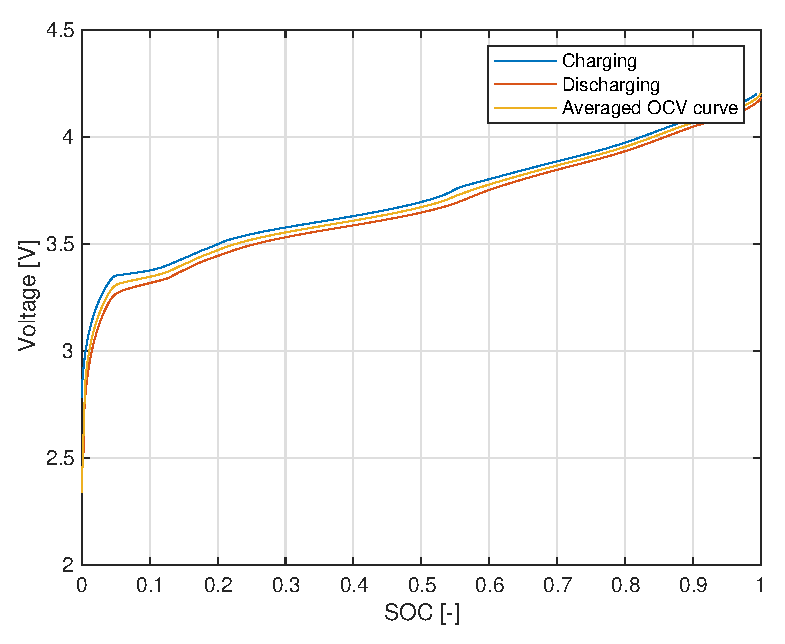
\includegraphics{figures/6/ocv.eps}
    \caption{Open circuit voltage as a function of SOC}
    \label{fig:6-ocv}
\end{figure}

\section{Identification of equivalent circuit model}

Estimated battery parameters are shown in Tab. \ref{tab:6-parameters}. The model achieved RMSE as low as 2.24 mV across the pulse experiment. This, combined with the degree of fit to training data shown in Fig. \ref{fig:6-pulse-compare} that is more than 86 \%, proves that the model indeed converged to reasonable parameters -- at least under the restriction of only 1 RC element. Adding more complexity to the model would improve its descriptive power and it would better match the system behavior.

The manual implementation of the discretized model was validated with results shown in Fig. \ref{fig:6-pulse-verification}. Since the results match the automatic comparison performed by Matlab, the model is implemented correctly.

\begin{figure}
    \centering
    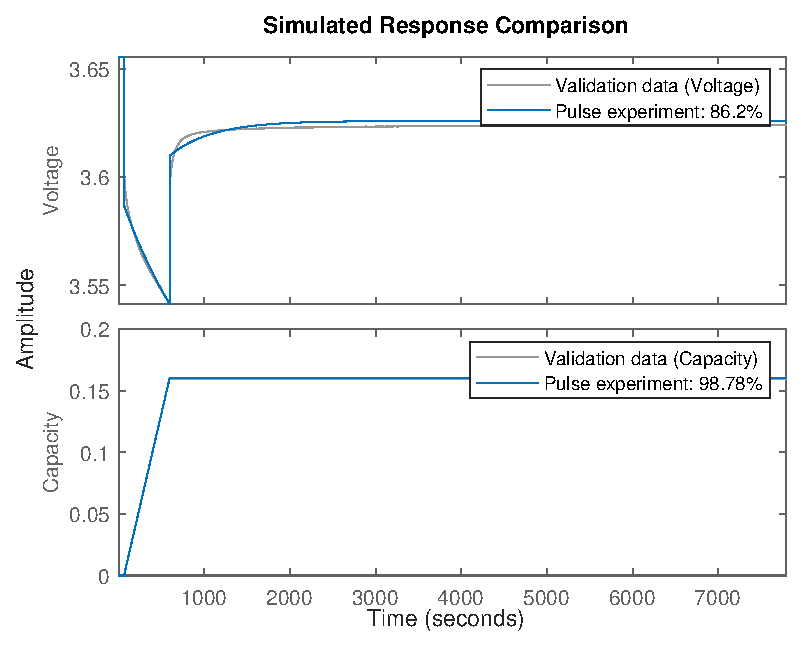
\includegraphics{figures/6/pulse-compare.eps}
    \caption{Assesment of model fit quality}
    \label{fig:6-pulse-compare}
\end{figure}

\begin{figure}
    \centering
    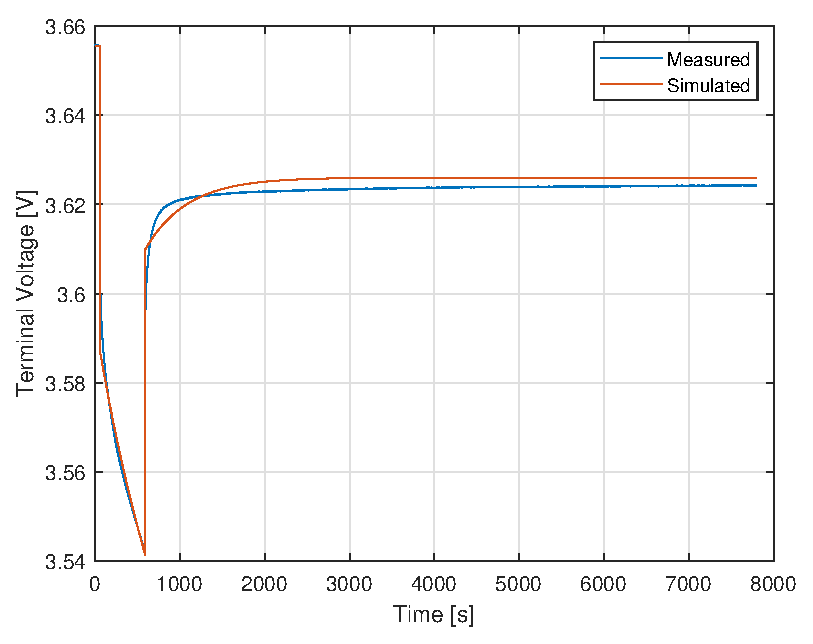
\includegraphics{figures/6/pulse-verification.eps}
    \caption{Manual comparison of model outputs and measurements}
    \label{fig:6-pulse-verification}
\end{figure}

\begin{table}[]
    \centering
    \begin{tabular}{c|c|c|c}
         Parameter & $R_0$ & $R_1$ & $C_1$ \\ \hline
         Value &  63.4e-3 $\Omega$ & 22.6e-3 $\Omega$ & 2.2e4 F 
    \end{tabular}
    \caption{Cell ECM parameters identified by the optimization procedure}
    \label{tab:6-parameters}
\end{table}

\section{Verification on dynamic discharge profile}

A provided DDP data set was used to verify model parameters identified in previous sections. The DDP consists of rapid discharge by constant 5.2 A, followed by discharge by 1.3 A and short charging by 2.5 A; everything in quick succession in 35 seconds. The model achieved RMSE of 47.3 mV across the whole experiment. Fig. \ref{fig:6-ddp-macro} shows that the model is indeed capable of capturing most of the cell dynamics, including gradual decrease of open circuit voltage. Some significant inaccuracy is still present however, as can be seen when zooming in on individual cycles of the DDP, as shown in Fig. \ref{fig:6-ddp-detail}. It is clear that the model failed to capture all system dynamics -- this is however expected since we have only used 1 RC element in the model. Adding a second one would improve the model fit to training data and decrease the RMSE on verification data. 

\begin{figure}
    \centering
    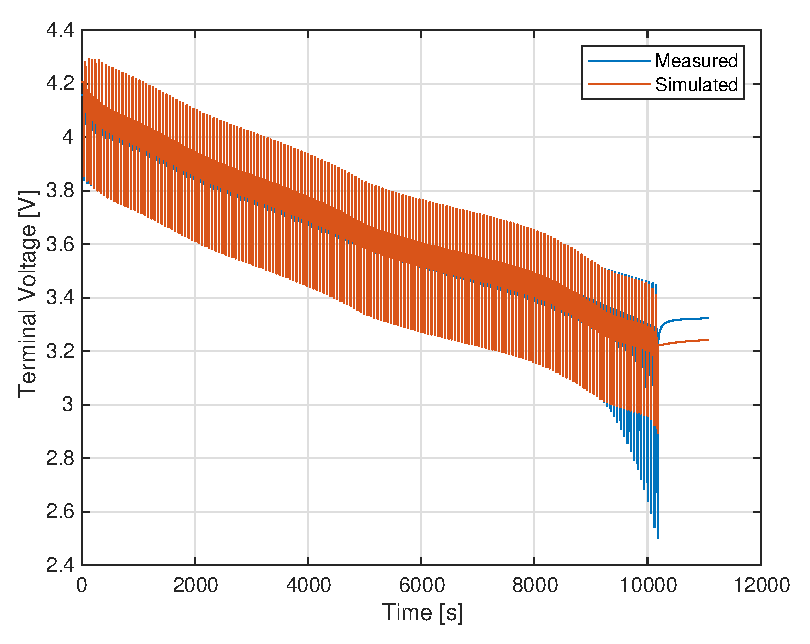
\includegraphics{figures/6/ddp-macro.eps}
    \caption{Comparison of measurements with simulated model outputs}
    \label{fig:6-ddp-macro}
\end{figure}

\begin{figure}
    \centering
    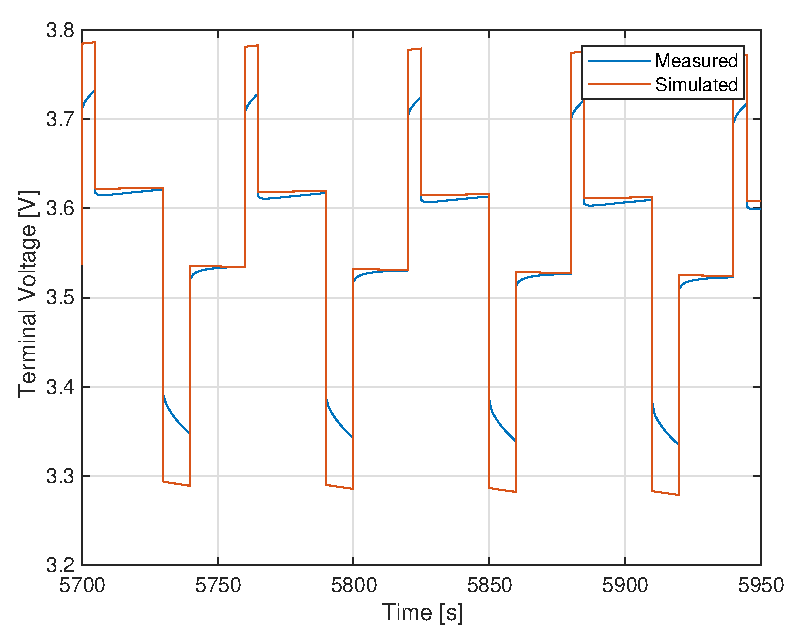
\includegraphics{figures/6/ddp-detail.eps}
    \caption{Verification of identified model on detail of several DDP cycles}
    \label{fig:6-ddp-detail}
\end{figure}



\chapter{Week 7 -- SOC Estimation, part 1}

\section{Abstract}
This report presents an implementation of several basic algorithms used for state-of-charge estimation. Using noisy input-output data from a simulation of a 2RC equivalent circuit model,
three methods of SoC determination -- namely the Coulomb counting, lookup using filtered terminal voltage and the combination of both -- were implemented and validated against reference data. All algorithms are executed for various values of hyperparameters to assess their robustness and errors caused by gradual drift or deviation in initial conditions. The accuracy of estimation is measured using the root-mean-square error.

\section{Cell model}

The chosen battery model considers only the dynamics of the $SoC$ and otherwise represents the cell as a static system
\begin{equation}
    \begin{split}
        \dot{SoC} &= -\frac{1}{C} i, \\
        \Ubat &= \OCV(SoC) - i R_0(SoC),
    \end{split}
    \label{eq:7-cont}
\end{equation}
with nonlinear output equation, where the system input $i$ denotes the flowing current, state $SoC \in \left[0, 1\right]$ is the state of charge, $\Ubat$ is the battery terminal voltage (system output) and the total capacity $C$, open circuit voltage $\OCV(SoC)$ and internal resistance $R_0(SoC)$ are (possibly $SoC$-dependent) model parameters. Numeric values of all model parameters are provided as a part of the assignment. Forward Euler discretization of \eqref{eq:7-cont} with sampling period $T_s = \SI{0.1}{\second}$ yields a simple system
\begin{equation}
    \begin{split}
        SoC(k+1) &= SoC(k) - \alpha \frac{T_s}{C} i(k), \\
        \Ubat(k) &= \OCV(SoC(k)) - i(k) R_0(SoC(k)),
    \end{split}
    \label{eq:7-disc}
\end{equation}
appropriate for the implementation in code. The state equation was extended with a scaling factor $\alpha$ that handles the conversion of capacity $C$ from ampere-hours to coulombs and the transformation of $SoC$ from $\left[0, 1\right]$ to percentage.

\begin{figure}
    \centering
    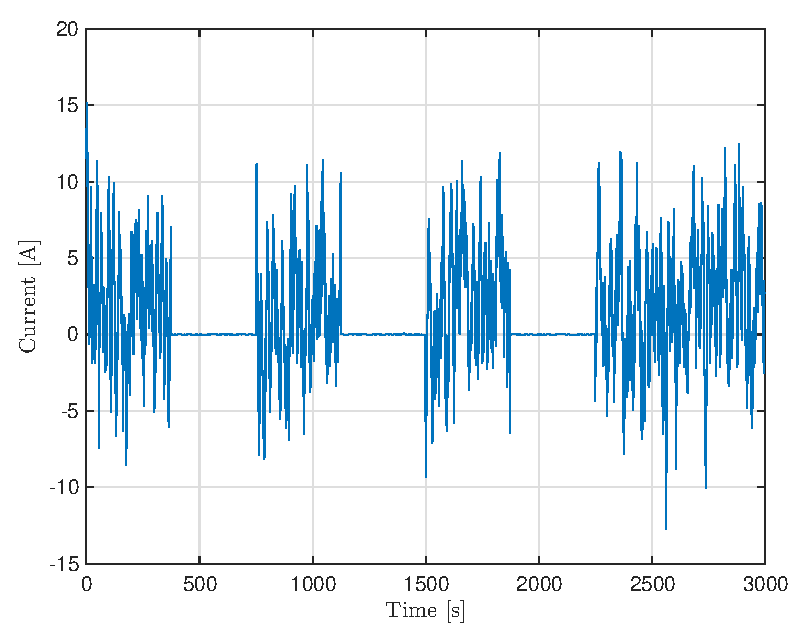
\includegraphics[width=0.5\textwidth]{figures/7/validation-I.eps}
    \caption{Current waveform used during all simulations.}
    \label{fig:7-validation-I}
\end{figure}

\section{Algorithm implementation}

The implementation was verified by simulating the model using provided parameter values and several sets of initial conditions and comparing them against waveforms obtained during the reference experiment. As shown in Fig. \ref{fig:7-validation-I}, the reference current represents a highly dynamic profile that combines high charging and discharging currents interleaved by several minutes-long rest periods with no current flow. This waveform is appropriate for demonstrating various SoC estimation algorithms as it excites both long-term and short-term cell dynamics.



\begin{figure}
    \centering
    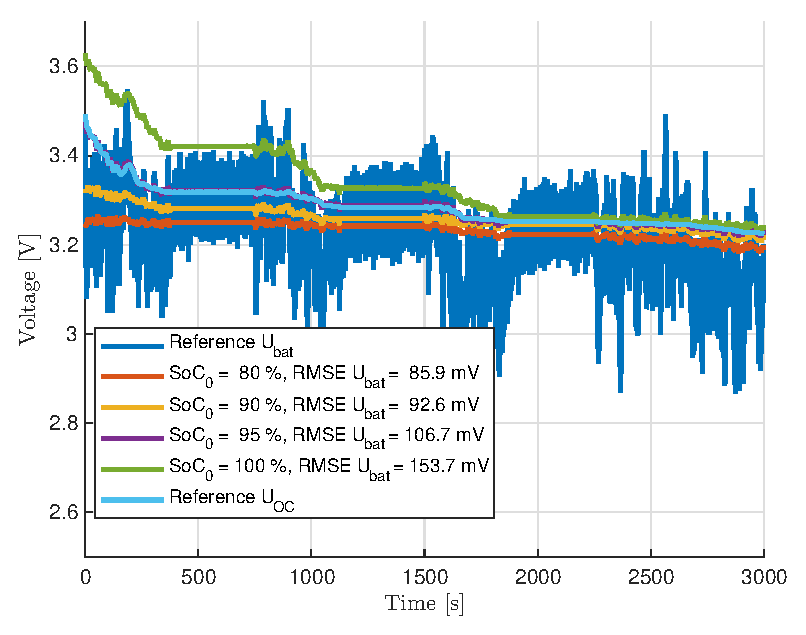
\includegraphics[width=0.5\textwidth]{figures/7/validation-Ubat.eps}
    \caption{Comparison of battery terminal voltages during simulation and the reference experiment.}
    \label{fig:7-validation-Ubat}
\end{figure}

Since the model \eqref{eq:7-disc} is very simple, large discrepancies between the reference waveform and simulation outputs are expected, as shown in Fig. \ref{fig:7-validation-Ubat}. Simulated terminal voltages differ by more than 80 mV using the RMSE metric, as they do not follow relatively fast dynamics observable in the reference waveform. The reason becomes apparent on closer inspection -- reference waveforms were generated using the 2RC equivalent circuit model, whereas the simulation only uses $R_0$ (neglecting $R_1$ and $R_2$). Neglecting the voltage drop across these resistances results in a far lower magnitude of voltage ripple in response to dynamically varying current.

\subsection{Coulomb counting}
\label{sec:7-cc}

The aforementioned systematic error is not a major issue for simple estimation of $SoC$, which, in the simple case without state observers, is completely unaffected by incorrect model impedance.The \textit{Coulomb counting} algorithm evaluates the state equation in \eqref{eq:7-disc}, performing an inherently open-loop integration of the flowing current. This way $SoC$ can be calculated without any knowledge about $\Ubat$, making this method useful when only a low-fidelity model is available.

\begin{figure}[bp]
    \centering
    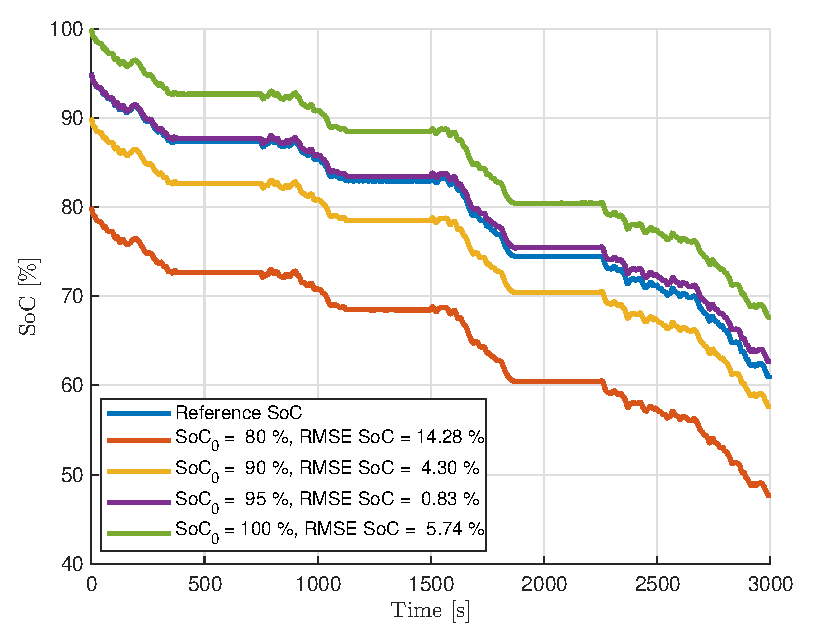
\includegraphics[width=0.5\textwidth]{figures/7/validation-SOC.eps}
    \caption{Comparison of simulated SoCs with the reference experiment.}
    \label{fig:7-validation-SOC}
\end{figure}

This is illustrated in Fig. \ref{fig:7-validation-SOC} -- since the $SoC$ evolution only depends on the accuracy of current measurement $i$ and cell capacity $C$ (and the coulombic efficiency $\eta$ when not neglected), estimates of $SoC$ for various initial conditions evolve "in parallel" and the error neither shrinks nor grows over time. However, even when the algorithm is initialized very close to the true initial state of charge (roughly 95 \%), it tends to drift away over time. Open-loop integration accumulates errors and has no means of self-correction.







\begin{figure}[tbp]
    \centering

\begin{subfigure}{0.49\textwidth}
    \centering
    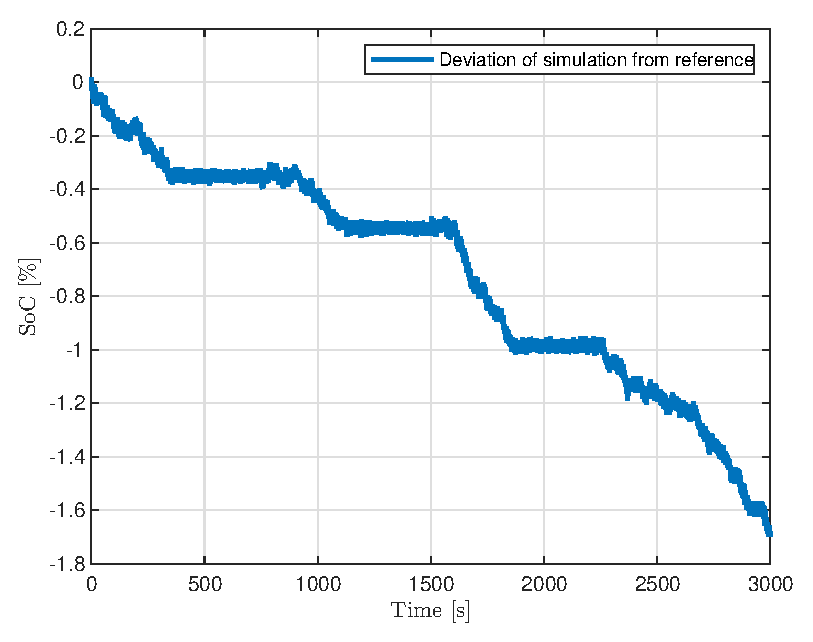
\includegraphics[width=\textwidth]{figures/7/validation-deviation-in-time.eps}
    \caption{Plotted over time.}
    \label{fig:7-validation-deviation-in-time}
    \end{subfigure}
    \hfill
    \begin{subfigure}{0.49\textwidth}
    \centering
    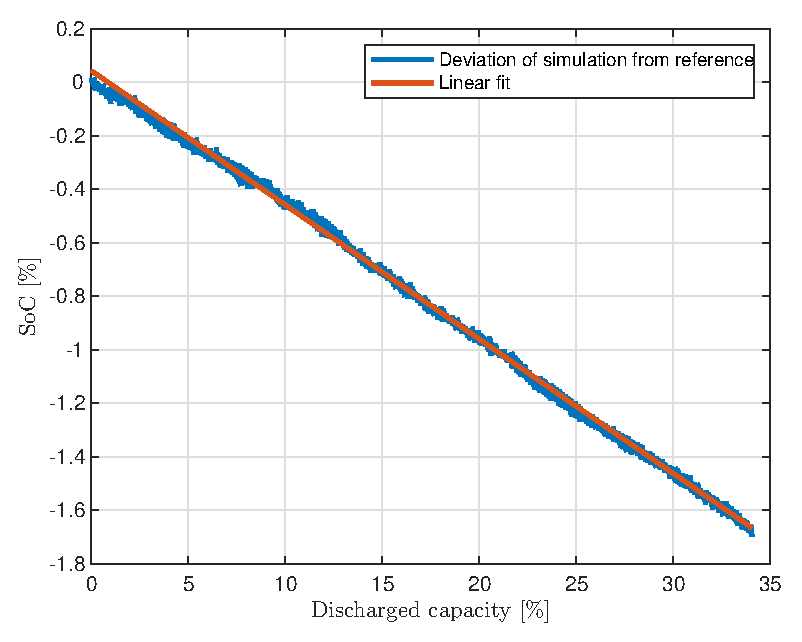
\includegraphics[width=\textwidth]{figures/7/validation-deviation.eps}
    \caption{Plotted w.r.t the Depth of Discharge (DoD).}
    \label{fig:7-validation-deviation}
    \end{subfigure}
    
    \caption{Gradual deviation of the reference and simulated SoC.}
    \label{fig:7-deviation}
\end{figure}

This behaviour can be observed in detail on Fig. \ref{fig:7-deviation}. Several possible factors may cause the simulated waveform to drift away from the reference $SoC$ over the course of the experiment, as shown in Fig. \ref{fig:7-validation-deviation-in-time}. Some insight into probable causes of the drift can be gained by looking at Fig. \ref{fig:7-validation-deviation}, where the error is plotted against the percentage of capacity discharged. Observing the highly linear dependence (linear fit achieves RMSE only 0.016 \% $SoC$), one can conclude that the error is purely multiplicative and hence could be fixed by recalibrating the current sensor, recalculating the cell capacity $C$ or possibly by extending the model with coulombic efficiency $\eta$, as the simulated output tends to overestimate the amount of charge remaining in the battery.

\subsection{Open circuit voltage lookup}
\label{sec:7-ocv}

\begin{figure}[b]
\centering
\begin{minipage}{0.49\textwidth}
    \centering
    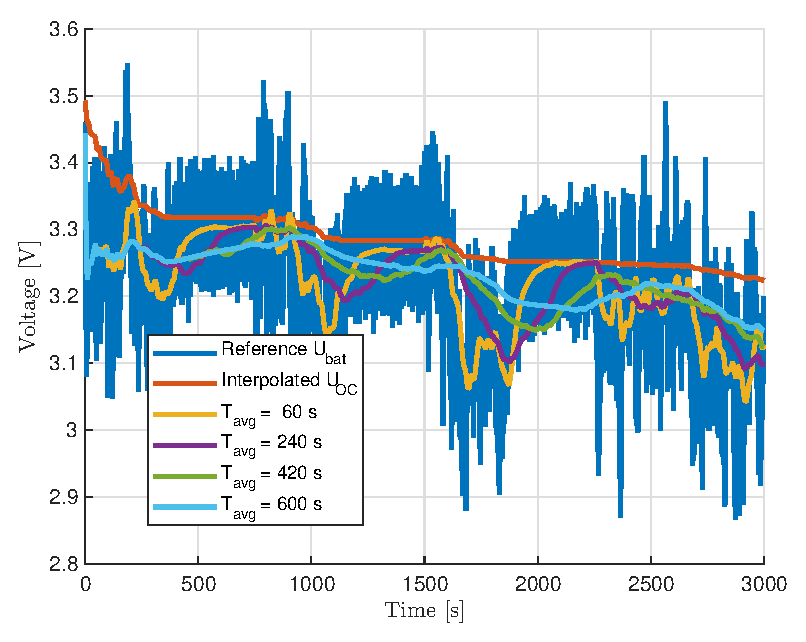
\includegraphics[width=\textwidth]{figures/7/OCV-Ubat.eps}
    \caption{$\OCV$ estimates for various values of $T_\text{avg}$.}
    \label{fig:7-OCV-Ubat}
\end{minipage}
\hfill
\begin{minipage}{0.49\textwidth}
    \centering
    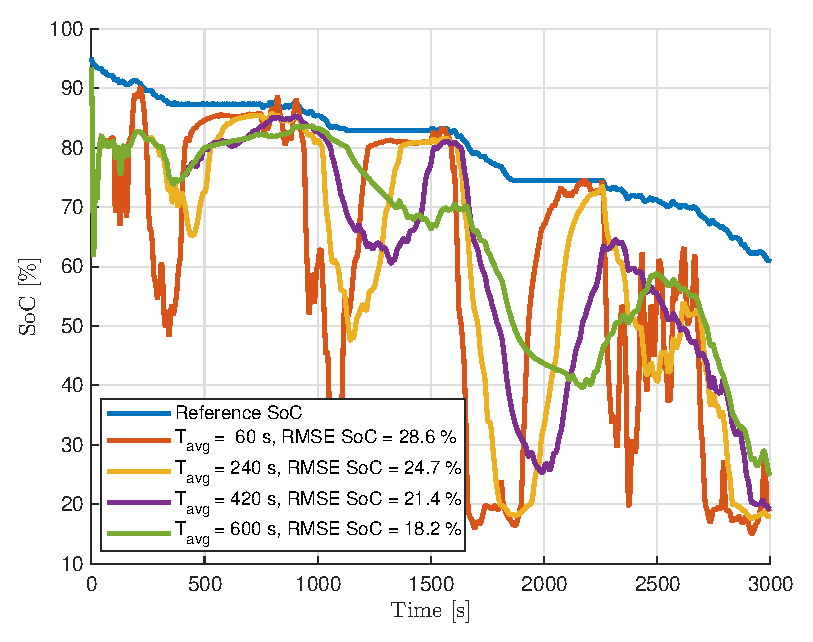
\includegraphics[width=\textwidth]{figures/7/OCV-SOC.eps}
    \caption{SoC estimates for various values of $T_\text{avg}$.}
    \label{fig:7-OCV-SOC}
\end{minipage}

\end{figure}

In contrast to Coulomb counting utilizing the measurement of battery current only, an alternative method uses only the measurement of battery terminal voltage $\Ubat$. Calculating a moving average of length $\Tavg$ over the recorded $\Ubat$ yields an approximation of the $\OCV$ that is subsequently used as an argument for table lookup.
Fig. \ref{fig:7-OCV-Ubat} shows how well the algorithm approximates the actual $\OCV$ with various setting of the hyperparameter $\Tavg$. A clear trend manifests, i.e. when $\Tavg$ is shorter, the algorithm is incapable of rejecting fast voltage drops when the cell is loaded, but it recovers quite quickly during the resting period. On the other hand, using a long averaging period $\Tavg$ results in stable $\OCV$ estimates (dynamically varying current goes through heavier filtering), but the approximation never approaches the actual $\OCV$ since averaging is longer than the resting period.

The same conclusion can be made when looking at Fig. \ref{fig:7-OCV-SOC} presenting $SoC$ estimates for various values of the hyperparameter $\Tavg$. Shorter $\Tavg$ yields an estimate with a larger variance that recovers quickly once the cell is allowed to rest. Longer $\Tavg$ ensures proper filtration of the estimate but simultaneously causes the estimate's mean value to deviate from the actual $SoC$. In this case, the algorithm underestimates the actual $SoC$ since the reference waveform reaches higher discharge currents than charging currents; therefore, the mean of $\Ubat$ is lower than $\OCV$.





\subsection{Coulomb counting with reset}
\label{sec:7-ccr}

Advantages of both previously analyzed algorithms can be merged to achieve the great stability of Coulomb counting and the robustness to incorrect initial conditions characteristic to the $\OCV$ lookup. The combined algorithm, from now on denoted as \textit{Coulomb counting with reset}, integrates the flowing current just like normal Coulomb counting. But whenever a resting period longer than $\Tdelay$ is detected, the measured terminal voltage $\Ubat$ is used as $\OCV$ to correct the $SoC$ estimate, removing any accumulated error.

\begin{figure}[htbp]
    \centering

\begin{subfigure}{0.49\textwidth}
    \centering
    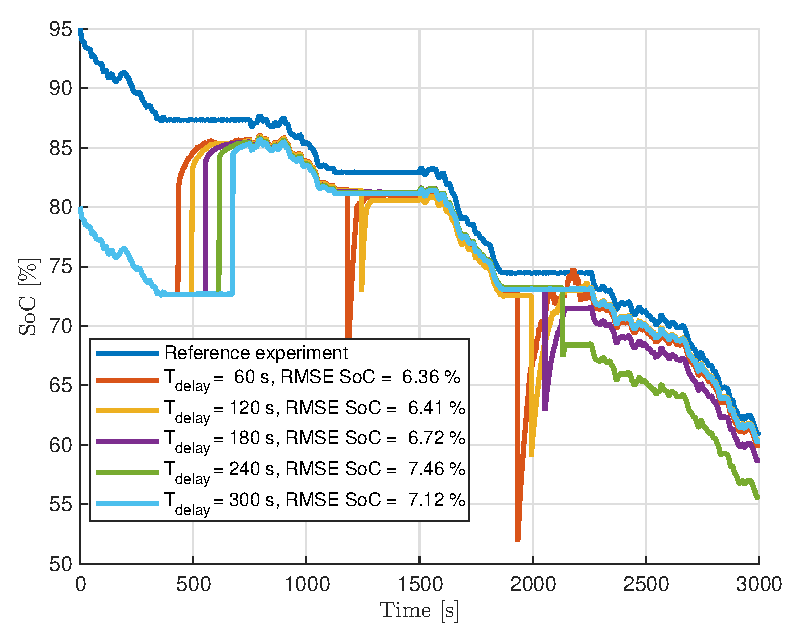
\includegraphics[width=\textwidth]{figures/7/combination-SOC.eps}
    \caption{SoC estimates for various hyperparameter values $T_\text{avg}$.}
    \label{fig:7-combination-SOC-macro}
    \end{subfigure}
    \hfill
    \begin{subfigure}{0.49\textwidth}
    \centering
    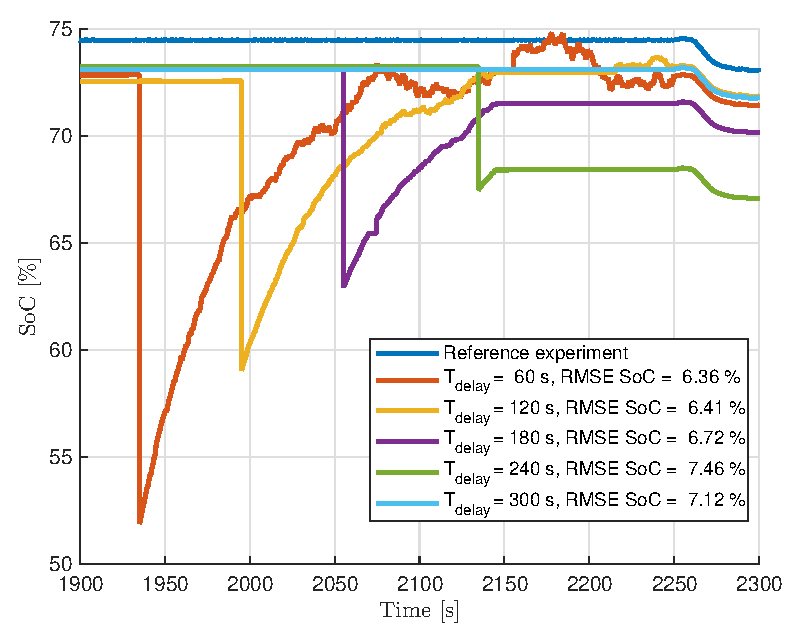
\includegraphics[width=\textwidth]{figures/7/combination-SOC-detail.eps}
    \caption{Detailed demonstration of reset behavior for various $T_\text{avg}$.}
    \label{fig:7-combination-SOC-detail}
    \end{subfigure}
    
    \caption{Demonstration of the \textit{Coulomb counting with reset} algorithm.}
    \label{fig:7-combination-SOC}
\end{figure}

This method has a hyperparameter $\Tdelay$, whose influence is illustrated in Fig. \ref{fig:7-combination-SOC}. When the current flow is interrupted at $t \approx \SI{380}{\second}$ and the cell is allowed to rest, $\Tdelay$ in some sense determines the amount of time given to the terminal voltage $\Ubat$ to converge to $\OCV$. After this delay elapses, the algorithm assumes that the $\Ubat$ has settled and uses its value to reset the integration.
The general trend regarding $\Tdelay$ can be inferred from Fig. \ref{fig:7-combination-SOC-detail} -- when the value gets larger,
the $SoC$ estimate is smoother (more filtered and less prone to short-term random walks), but extending $\Tdelay$ to infinity is not useful, as once it becomes longer than any reasonable resting period, the algorithm degenerates back to pure Coulomb counting without resets.
On the other hand, shorter $\Tdelay$ results in more frequent resets of the coulomb counting algorithm that occur even when $\Ubat$ is not fully settled, causing unwanted downwards spikes visible across the whole experiment in Fig. \ref{fig:7-combination-SOC-macro}.


\begin{figure}
    \centering
    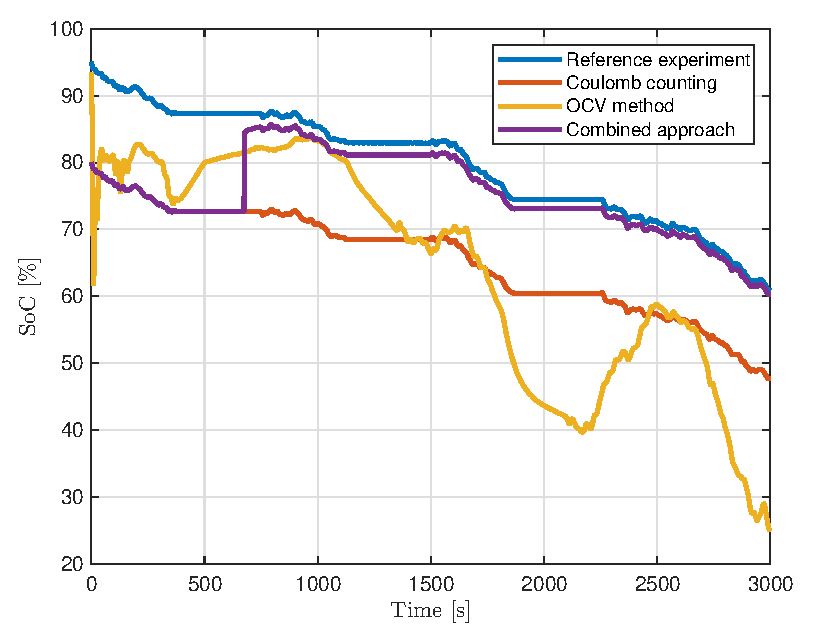
\includegraphics[width=0.5\textwidth]{figures/7/comparison-SOC.eps}
    \caption{Performance comparison of presented estimation algorithms.}
    \label{fig:7-comparison-SOC}
\end{figure}

\section{Discussion}

In this homework, three simple methods of state-of-charge estimation were implemented. The first one -- Coulomb counting -- directly repeatedly evaluates the state equation for $SoC$ using the current measurement $i$. The second method approximates $\OCV$ by filtering terminal voltage measurement $\Ubat$ and subsequently looks the $SoC$ up in a static table. The third method combines both approaches by performing Coulomb counting with occasional resets of the integrator with a value approximated using the $\OCV$.

Key differences between methods can be identified by inspecting Fig. \ref{fig:7-comparison-SOC}, where each method is represented by just one waveform. Each selected waveform does not necessarily minimize the $SoC$ RMSE, but it displays characteristic behavior and disadvantages inherent to the used method. The OCV method, as implemented in Sec. \ref{sec:7-ocv}, leads generally to the "wildest" (and worst) estimate from the customer's point of view. Coulomb counting analyzed in Sec. \ref{sec:7-cc} leads to very accurate estimates of $\Delta SoC$ over short time periods before the integration accumulates significant errors. It is however incapable of yielding absolute $SoC$, since the initial condition for integration is unknown in real applications. Clearly the best performance is achieved by the combined algorithm discussed in Sec. \ref{sec:7-ccr}, because it combines infrequent updates about the absolute $SoC$ from the OCV method with high accuracy relative $\Delta SoC$ calculated by the Coulomb counting.

This conclusion is supported by comparison of root-mean-square errors of estimates; as shown in Fig. \ref{fig:7-validation-SOC}, Coulomb counting is capable of achieving very low RMSE when given exact knowledge of the initial value. The OCV method achieves RMSE of roughly 18 \% or more, as shown in Fig. \ref{fig:7-OCV-SOC}, but it does not depend on the algorithm's initialization. Finally the values in Fig. \ref{fig:7-combination-SOC} show what the combined approach achieves errors as low as 7 \% in spite of very wrong initial estimate of $SoC$. Coulomb counting with reset combines low RMSE of Coulomb counting and robustness to wrong initial conditions characteristic to the OCV method.


\chapter{Week 8 -- SOC Estimation -- Extended Kalman Filter}

\section{Abstract}
This report presents an implementation of an EKF-based algorithm for state-of-charge estimation and compares its performance with several simple methods implemented in the previous assignment. Using noisy input-output data from a simulation of a 2RC equivalent circuit model,
the nonlinear discrete-time 2RC equivalent circuit model is validated. This model is subsequently linearized analytically around a general operating point to obtain matrices $\mathbf{A}$ and $\mathbf{C}$ needed by the Extended Kalman Filter. Tuning noise covariance matrices $\mathbf{Q}$ and $\mathbf{R}$ is discussed. The performance of EKF is compared to simpler methods, namely the Coulomb counting, table lookup using filtered terminal voltage and a combination of both. Methods are compared visually as well as quantitatively using the root-mean-square error.

\section{Model implementation and validation}
\label{sec:8-one}

The chosen implemented battery model is the standard 2RC equivalent circuit model
\begin{align}
        \dot{U_1} &= -\frac{1}{R_1 C_1} U_1 + \frac{1}{C_1} i, \label{eq:8-cont1} \\
        \dot{U_2} &= -\frac{1}{R_2 C_2} U_2 + \frac{1}{C_2} i, \\
        \dot{SoC} &= -\frac{100}{C} i, \\
        \Ubat &= \OCV(SoC) - U_1 - U_2 - R_0i,
    \label{eq:8-cont4}
\end{align}
with a nonlinear output equation, where the system input $i$ denotes the flowing current, states $U_1$ and $U_2$ are voltage drops across the two RC elements, $SoC \in \left[0, 100\right]$ \% is the state of charge, $\Ubat$ is the battery terminal voltage (system output) and the total capacity $C$, open circuit voltage $\OCV(SoC)$, resistances $R_{0,1,2}$ and capacitances $C_{1,2}$ are (possibly $SoC$-dependent) model parameters with numeric values provided as a part of the assignment. To facilitate a simple iterative simulation of system behavior, the system \eqref{eq:8-cont1}-\eqref{eq:8-cont4} was discretized using the Forward Euler method as
\begin{equation}
\begin{split}
    x(k+1) &= x(k) + T_s f(x(k), u(k)), \\
    y(k) &= g(x(k), u(k)),
\end{split}
\label{eq:8-disc}
\end{equation}
where $f$ and $g$ are vector functions of right-hand sides of \eqref{eq:8-cont1}-\eqref{eq:8-cont4} and $x(k)$, $u(k)$ and $y(k)$ are the system state, input and output vector at sample $k$, respectively.

\begin{figure}[H]
    \centering
    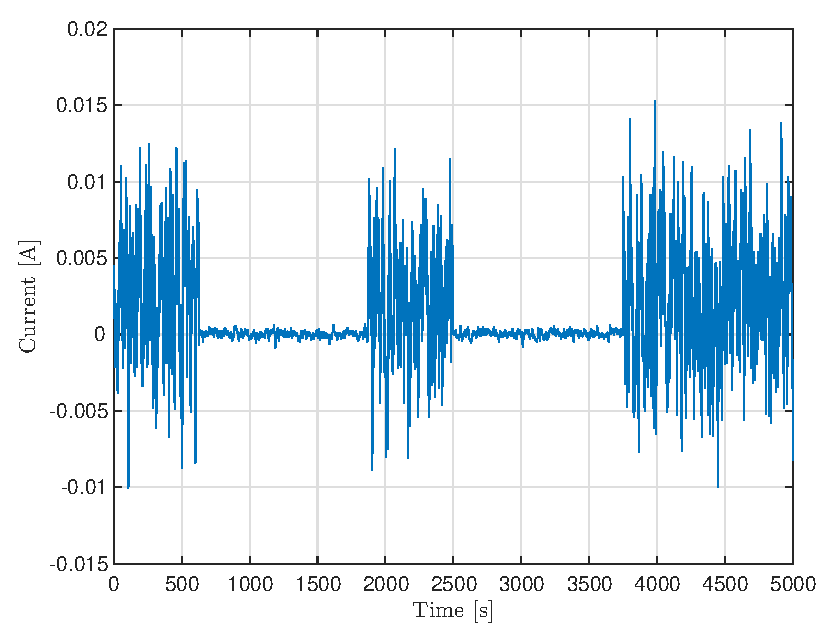
\includegraphics[width=0.5\textwidth]{figures/8/validation-I.eps}
    \caption{Current waveform used during all simulations.}
    \label{fig:8-validation-I}
\end{figure}

The same current waveform shown in Fig. \ref{fig:8-validation-I} that was recorded during the reference experiment was used for all simulations. Results of simulation with \eqref{eq:8-disc} are shown in Fig. \ref{fig:8-validation}, specifically Fig. \ref{fig:8-validation-SOC} shows the evolution of system state $SoC$ whereas Fig. \ref{fig:8-validation-U} compares the reference and simulated system output. Results confirm the expected near-perfect match of reference and simulated signals, since the reference experiment itself was a simulation, presumably using identical model parameters.

\begin{figure}[hbp]
    \centering
\begin{subfigure}{0.49\textwidth}
    \centering
    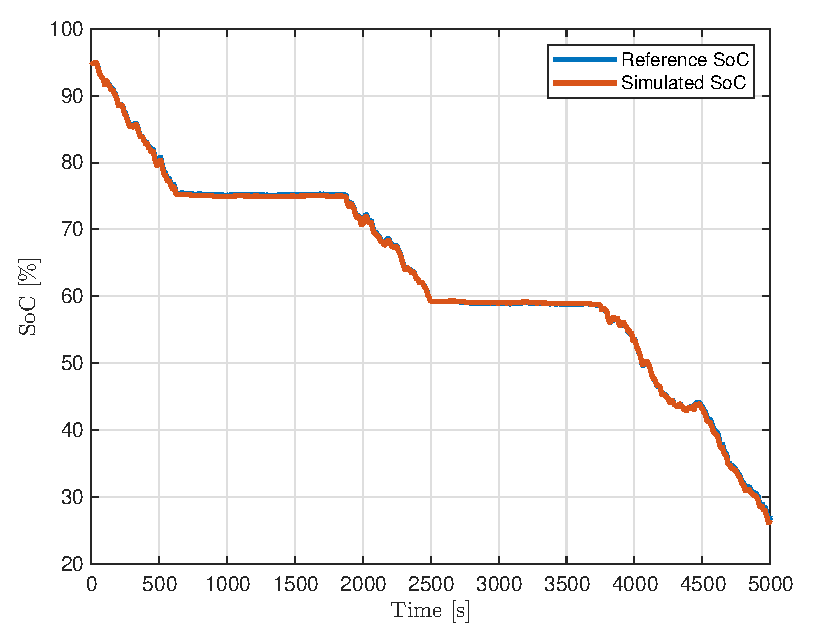
\includegraphics[width=\textwidth]{figures/8/validation-soc.eps}
    \caption{State of charge $SoC$.}
    \label{fig:8-validation-SOC}
    \end{subfigure}
    \hfill
    \begin{subfigure}{0.49\textwidth}
    \centering
    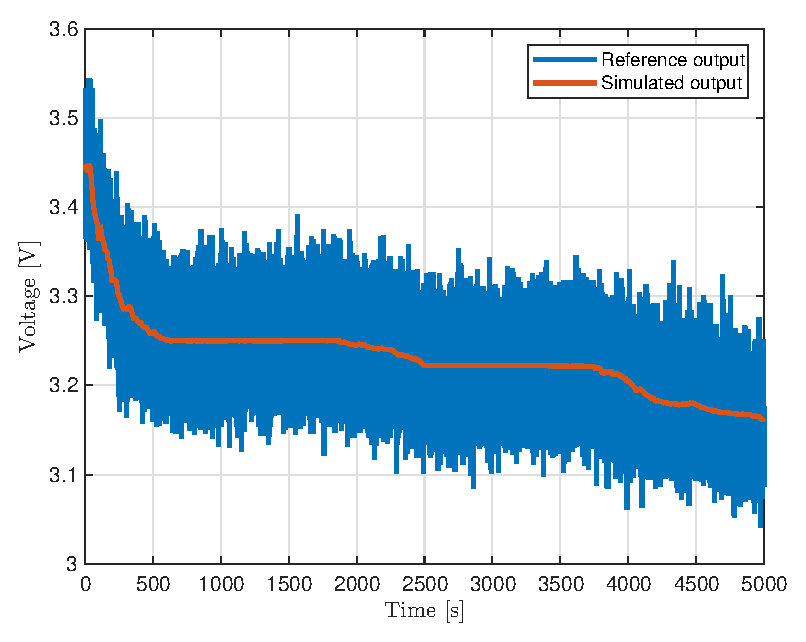
\includegraphics[width=\textwidth]{figures/8/validation-U.eps}
    \caption{Terminal voltage $\Ubat$.}
    \label{fig:8-validation-U}
    \end{subfigure}
    
    \caption{Comparison of reference and simulated waveforms.}
    \label{fig:8-validation}
\end{figure}

Assuming that the discrepancy between the simulated and reference $\Ubat$ visible in Fig. \ref{fig:8-validation-U} is purely an additive noise sequence $e$, its parameters can be extracted. The random sequence $e$ has zero mean and variance $\sigma^2 \approx 0.0013$. To assess its whiteness, its normalized autocorrelation function was evaluated and plotted in Fig. \ref{fig:8-validation-pred-error}. Since the correlation for any lag other than 0 samples is far below the 5 \% threshold, the noise sequence $e$ can be assumed white. This result is relevant for the theoretical justification of the correctness of results obtained by the Kalman Filter.


\begin{figure}[hbp]
    \centering
\begin{subfigure}{0.49\textwidth}
    \centering
    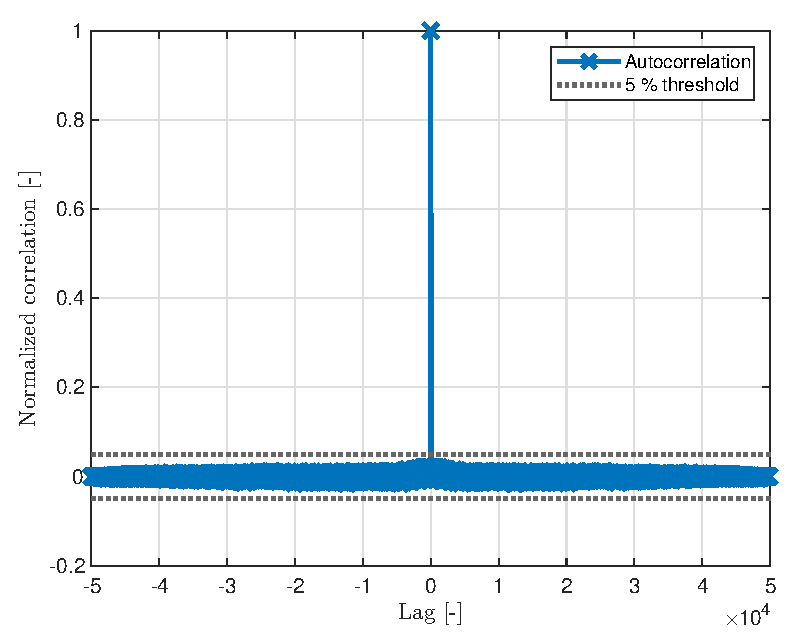
\includegraphics[width=\textwidth]{figures/8/validation-pred-error.eps}
    \caption{For all possible shifts of the signal}
    \label{fig:8-validation-pred-error-global}
    \end{subfigure}
    \hfill
    \begin{subfigure}{0.49\textwidth}
    \centering
    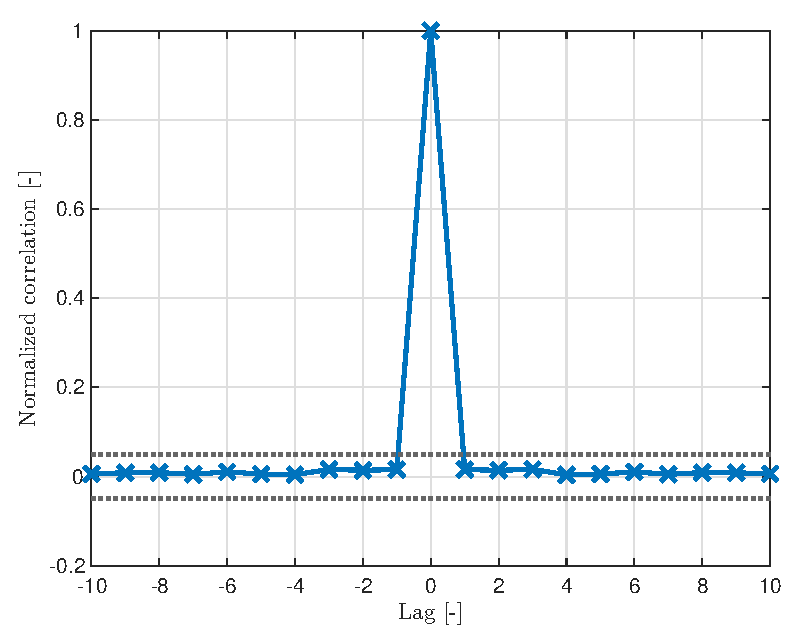
\includegraphics[width=\textwidth]{figures/8/validation-pred-error-detail.eps}
    \caption{Detail of the autocorrelation for low values of the signal lag}
    \label{fig:8-validation-pred-error-detail}
    \end{subfigure}
    
    \caption{Autocorrelation of the prediction error.}
    \label{fig:8-validation-pred-error}
\end{figure}

\section{EKF Implementation}

Building on top of the discrete-time model \eqref{eq:8-disc}, the Extended Kalman Filter was implemented. Apart from the state evolution and output functions, the algorithm requires their derivatives w.r.t. individual states to form time-varying Jacobian matrices
\begin{align}
    \mathbf{C}(k) &= \frac{\partial y(k)}{\partial x(k)}\biggr\rvert_{x(k),u(k)} &=& \begin{bmatrix} -1 & -1 & \frac{\partial \OCV(SoC(k))}{\partial SoC} \end{bmatrix}\biggr\rvert_{SoC(k)}, \\
        \mathbf{A}(k) &= \frac{\partial x(k+1)}{\partial x(k)}\biggr\rvert_{x(k),u(k)} = \mathbf{I} + T_s \frac{\partial f(x(k), u(k))}{\partial x(k)}\biggr\rvert_{x(k),u(k)} &=& \begin{bmatrix}
            1 - \frac{T_s}{R_1 C_1} & 0 & 0 \\ 0 & 1 - \frac{T_s}{R_2 C_2} & 0 \\ 0 & 0 & 1
        \end{bmatrix}.
\end{align}
Although the state matrix $\mathbf{A}$ is time invariant, the last element of the output matrix $\mathbf{C}(k)$ is the derivative of the cell's OCV curve that is highly dependent on the immediate $SoC(k)$. The necessity of existence of the partial derivative $\frac{\partial \OCV(SoC(k))}{\partial SoC}$ makes the lookup table implementation of the OCV curve disadvantageous and calls for a polynomial fit -- in this case approximation by a polynomial of the 5th degree shown in Fig. \ref{fig:8-ocv} together with its derivative.

\begin{figure}[H]
    \centering
    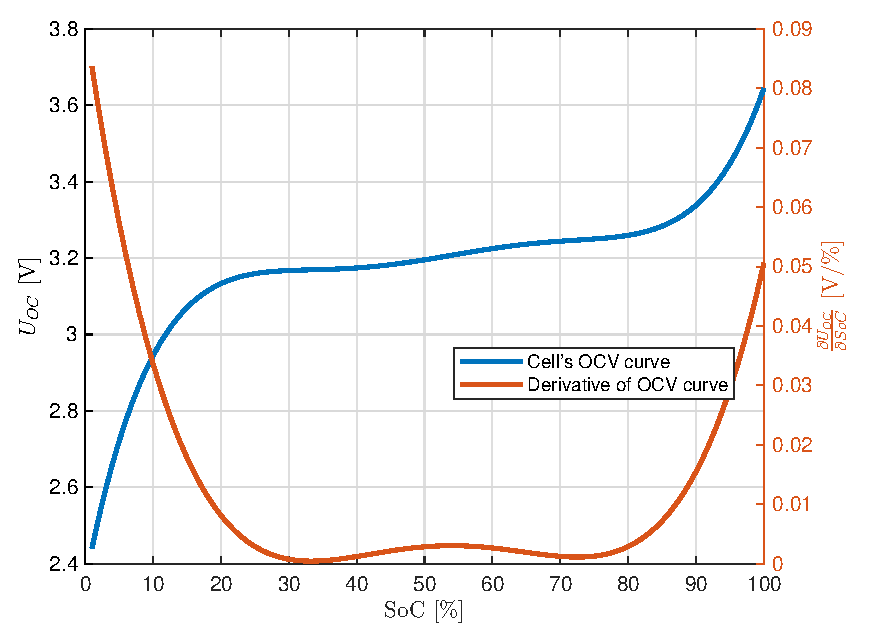
\includegraphics[width=0.5\textwidth]{figures/8/ocv_to_soc.eps}
    \caption{Polynomial approximations of the $\VOC$ curve and its derivative.}
    \label{fig:8-ocv}
\end{figure}

The single element of measurement noise covariance matrix $\mathbf{R}$ was already determined during the analysis of the additive measurement noise $e$ in Section \ref{sec:8-one} as $\mathbf{R} = \sigma^2 \approx 0.0013$. Tuning the process noise covariance matrix $\mathbf{Q}$ required several iterations and resulted in
\begin{equation}
    \mathbf{Q} = \begin{bmatrix}
    10^{-12} & 0 & 0 \\ 0 & 10^{-12} & 0 \\ 0 & 0 & 10^{-4}
\end{bmatrix}.
\end{equation}
Considering the range of reasonable values of system states and other quantities, elements of $\mathbf{Q}$ seem very small and this fact could lead to deterioration of computation accuracy. Should this ever become a problem, one could normalize system variables to obtain a more robust numerical stability. Nevertheless in this case one can easily justify matrix elements this small -- there is no reason to consider any noise apart from the additive measurement noise $e$ characterized by $\sigma^2$ that was calculated exactly using provided data. The process noise only has to cover unmodelled system dynamics. Due to symmetry, there is no reason to choose different values of variances corresponding to $U_1$ and $U_2$ and both should be far lower than the variance corresponding to $SoC$. This is because we want the EKF to primarily adjust the $SoC$ estimate to explain the observed output, whereas estimates of both polarization voltages $U_{i}$ should rely mostly on the model and should not be varied by the EKF to explain observed terminal voltages.

Results (estimates) given by the EKF are shown in Fig. \ref{fig:8-ekf}. Great gradual convergence to the true state of charge is shown in Fig. \ref{fig:8-ekf-soc}, whereas Fig. \ref{fig:8-ekf-U} shows great rejection of the additive measurement noise, as the predicted output voltage almost perfectly matches the noiseless reference output with RMSE as low as 16 mV when calculated globally and only 4 mV when calculated from $t = 2000$ onwards, where the filter has perfectly converged to the true state.

\begin{figure}[H]
    \centering
\begin{subfigure}{0.49\textwidth}
    \centering
    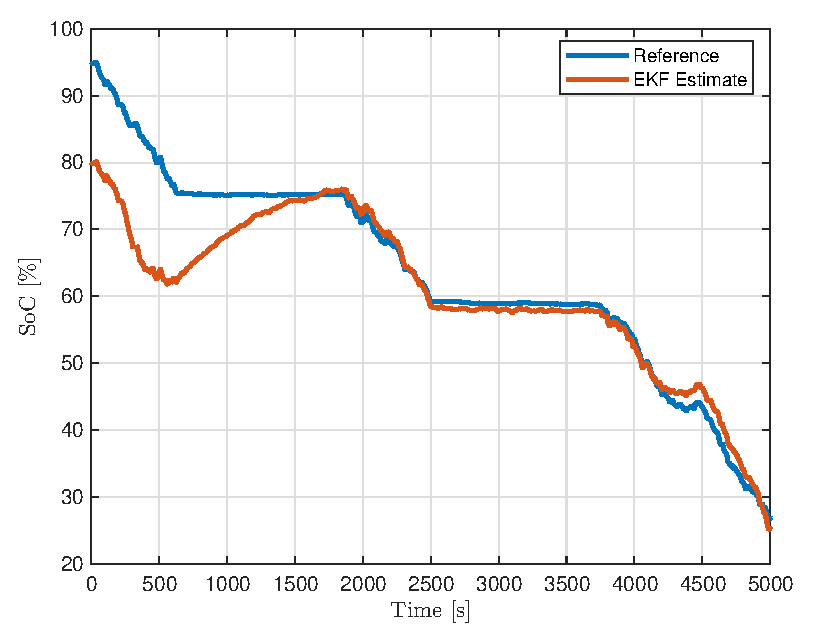
\includegraphics[width=\textwidth]{figures/8/ekf-soc.eps}
    \caption{State of charge $SoC$.}
    \label{fig:8-ekf-soc}
    \end{subfigure}
    \hfill
    \begin{subfigure}{0.49\textwidth}
    \centering
    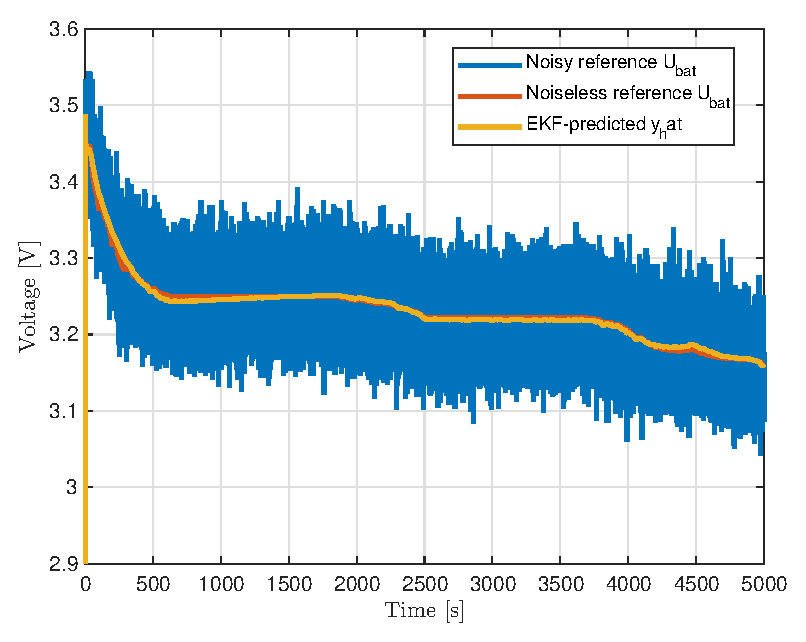
\includegraphics[width=\textwidth]{figures/8/ekf-U.eps}
    \caption{Terminal voltage $\Ubat$.}
    \label{fig:8-ekf-U}
    \end{subfigure}
    
    \caption{Comparison of reference waveforms with EKF estimates/predictions.}
    \label{fig:8-ekf}
\end{figure}

\section{Discussion}

This homework is a continuation of the previous report (HW7) that presented implementation and results for three simple methods of $SoC$ estimation. It presented many results and observations that will not be repeated, the reader is therefore advised to read its conclusions  before proceeding.

This report added a new $SoC$ estimation method based on the Extended Kalman Filter. All methods are compared in Fig \ref{fig:8-comparison} with results summarized in \ref{tab:8-comparison}. Compared to simple methods from the previous assignment, estimation by the Extended Kalman Filter enjoys a balance of robustness to the selection of initial conditions and accuracy of predicted system behavior. Observing Fig. \ref{fig:8-comparison-dev}, one may conclude that
\begin{enumerate}
    \item Even when the EKF is started with incorrect initial conditions, it eventually converges to the correct solution (unlike the Coulomb counting method), and
    \item once the EKF converges to the reference value, it never deviates far (unlike the $\OCV$ lookup method).
\end{enumerate}

\begin{figure}[hbp]
    \centering
\begin{subfigure}{0.49\textwidth}
    \centering
    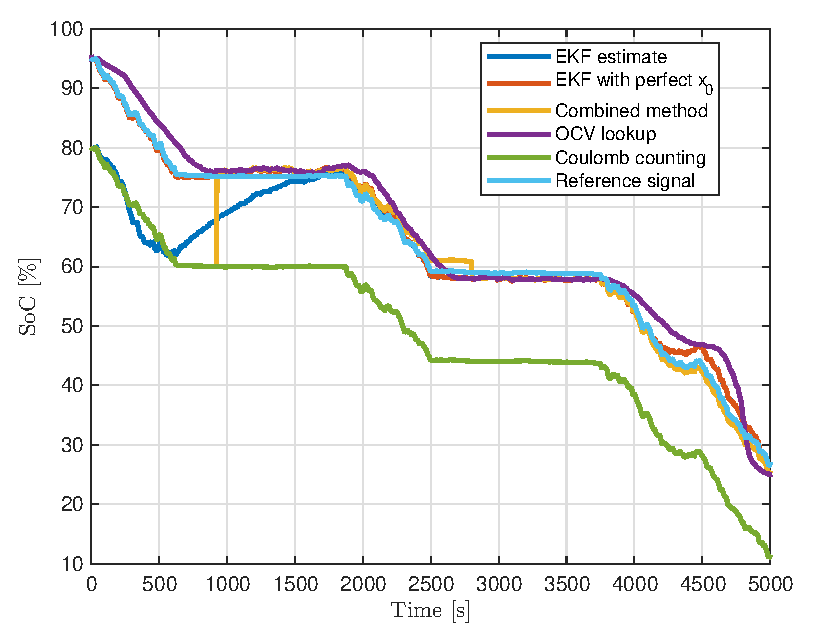
\includegraphics[width=\textwidth]{figures/8/comparison.eps}
    \caption{Absolute values of $SoC$ estimates.}
    \label{fig:8-comparison-abs}
    \end{subfigure}
    \hfill
    \begin{subfigure}{0.49\textwidth}
    \centering
    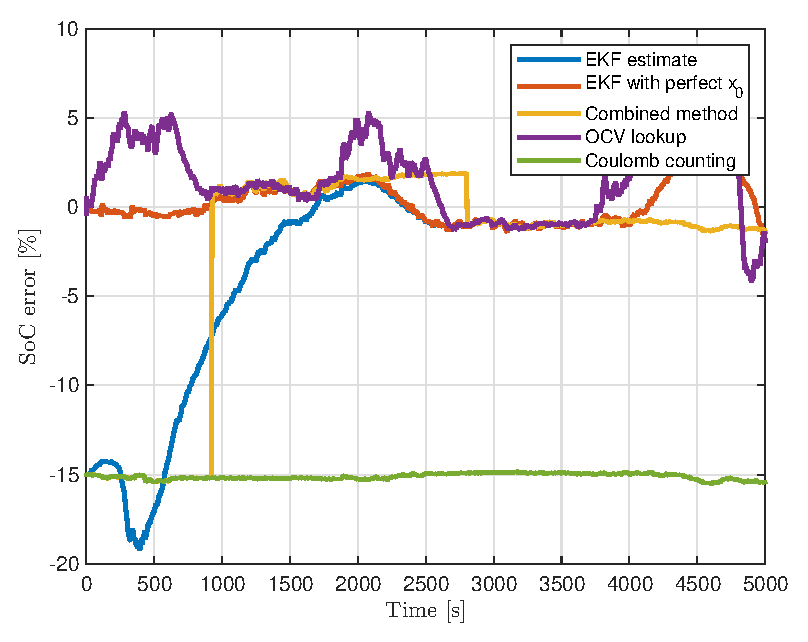
\includegraphics[width=\textwidth]{figures/8/comparison-dev.eps}
    \caption{Deviations of $SoC$ estimates from the reference.}
    \label{fig:8-comparison-dev}
    \end{subfigure}
    
    \caption{Comparison of estimation performance of individual algorithms.}
    \label{fig:8-comparison}
\end{figure}

\begin{table}[t]
    \centering
    \begin{tabular}{c|c|c}
         Method & $SoC$ RMSE [\%]& $SoC$ RMSE [\%] for $t > 2000$ s \\ \hline
         Extended Kalman Filter & 6.45 & 1.38 \\
         Coulomb Counting & 15.11 & 15.04 \\
         $\OCV$ lookup & 2.93 & 3.14 \\
         Reset-Coulomb counting & 6.62 & 1.23 \\ \hline
         Extended Kalman Filter w/ perfect ICs & 1.19 & 1.40 \\
    \end{tabular}
    \caption{Errors of estimates yielded by various methods.}
    \label{tab:8-comparison}
\end{table}

Although the OCV-lookup method achieves the lowest RMSE on the whole experiment (with the exception of EKF with perfect knowledge of initial conditions), this is caused by its ultimate lack of dynamics -- if the mean of terminal voltage $\Ubat$ was subject to more dynamical changes (e.g. due to higher current $i$), the OCV lookup estimate would quickly deteriorate as the approximated $\OCV$ would be incorrect. On the other hand, the Coulomb counting has the clear disadvantage of no correction for imprecise knowledge of initial conditions. Coulomb counting with reset solves this problem, but the correction around $t \approx \SI{900}{\second}$ is too sudden and would certainly lead to customer dissatisfaction if it happened e.g. in a smartphone or an electric vehicle. Additionally the correction performed by the reset is only as good as the OCV-lookup method, disadvantages of which were already discussed in detail in the previous report.

For these reasons, the EKF algorithm is the winner in terms of quality of the resulting estimate. One should note however that the implementation of EKF is significantly more complex and computationally demanding than any of the simpler previously discussed methods.
The EKF estimate could be further improved e.g. by using a higher-order fit of the cell's $\OCV$ curve, since the currently used model seems to deviate a little from the true waveform for $SoC < 50$ \%.







\chapter{Week 9 -- SOH Estimation}

\section{Abstract}
This report presents an implementation of a dual-Extended Kalman Filter architecture used for state of health ($SoH$) estimation. An EKF for $SoC$ estimation using measured terminal voltage presented in the previous lab report is complemented by a second two-state EKF used for the estimation of battery capacity $C$ used to assess the state of health.

\section{Model implementation}
\label{sec:9-one}

The $SoH$ estimation architecture requires two separate models -- the battery and the slow aging process.
Just like in the previous assignment, the battery model was chosen as the standard 2RC equivalent circuit model
\begin{align}
        \dot{U_1} &= -\frac{1}{R_1 C_1} U_1 + \frac{1}{C_1} i, \label{eq:9-cont1} \\
        \dot{U_2} &= -\frac{1}{R_2 C_2} U_2 + \frac{1}{C_2} i, \\
        \dot{SoC} &= -\frac{100}{C} i, \\
        \Ubat &= \OCV(SoC) - U_1 - U_2 - R_0i,
    \label{eq:9-cont4}
\end{align}
with a nonlinear output equation, where the system input $i$ denotes the flowing current, states $U_1$ and $U_2$ are voltage drops across the two RC elements, $SoC \in \left[0, 100\right]$ \% is the state of charge, $\Ubat$ is the battery terminal voltage (system output) and the open circuit voltage $\OCV(SoC)$, resistances $R_{0,1,2}$ and capacitances $C_{1,2}$ are (possibly $SoC$-dependent) model parameters with numeric values provided as a part of the assignment. In this task the total capacity $C$ is not assumed constant and is estimated by the second EKF.
To facilitate a simple iterative simulation of system behavior, the system \eqref{eq:9-cont1}-\eqref{eq:9-cont4} was discretized using the Forward Euler method as
\begin{equation}
\begin{split}
    x(k+1) &= x(k) + T_s f(x(k), u(k)), \\
    y(k) &= g(x(k), u(k)),
\end{split}
\label{eq:9-disc}
\end{equation}
where $f$ and $g$ are vector functions of right-hand sides of \eqref{eq:9-cont1}-\eqref{eq:9-cont4} and $x(k)$, $u(k)$ and $y(k)$ are the system state, input and output vector at sample $k$, respectively.

Battery ageing is modelled as a gradual decrease of the available capacity $C$. There are no degradation dynamics modelled
\begin{align}
    C(k+1) &= C(k) + v_1(k), \\
    \hat{SoC}(k+1) &= \hat{SoC}(k) - \frac{1}{C(k)}i(k) + v_2(k),
\end{align}
hence any change in the battery capacity $C$ originates from the influence of process noise $v(k)$. The quantity $\hat{SoC}$ is a secondary estimate of battery $SoC$ calculated by the SoH-EKF. It acts as an output of the SoH-EKF that is compared to the $SoC$ estimate given by SoC-EKF to obtain the prediction error. This prediction error then drives the SoH-EKF to estimate the correct battery capacity.
\clearpage
\section{Experimental results}

Equations were implemented in code to verify that the model and provided parameters work correctly and can reproduce the reference waveforms. A comparison of reference (given) and my simulated signals is in Fig. \ref{fig:9-validation}. Signals clearly do not match, indicating a significant discrepancy in the provided model and model used to generate reference data.
Although many iterations of the trial and error method showed that part of the discrepancy is caused by the neglected Coulombic efficiency $\eta \approx 0.977$, it is not the only cause. It is -- for example -- not clear from the assignment, where in the cycle is the reference battery capacity (recorded as one sample per charge-discharge cycle) recorded. Apart from that, it is unspecified whether the capacity in the reference simulation is piecewise constant or linearly decreasing during the cycle. These uncertainties about the provided data result in significant errors in the result.


\begin{figure}[hbp]
    \centering
\begin{subfigure}{0.49\textwidth}
    \centering
    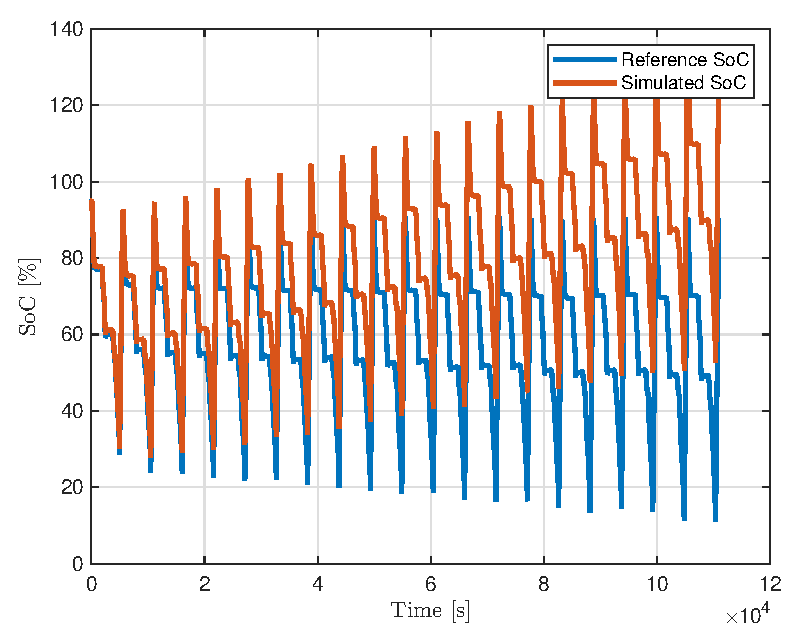
\includegraphics[width=\textwidth]{figures/9/validation-soc.eps}
    \caption{State of charge $SoC$.}
    \label{fig:9-validation-SOC}
    \end{subfigure}
    \hfill
    \begin{subfigure}{0.49\textwidth}
    \centering
    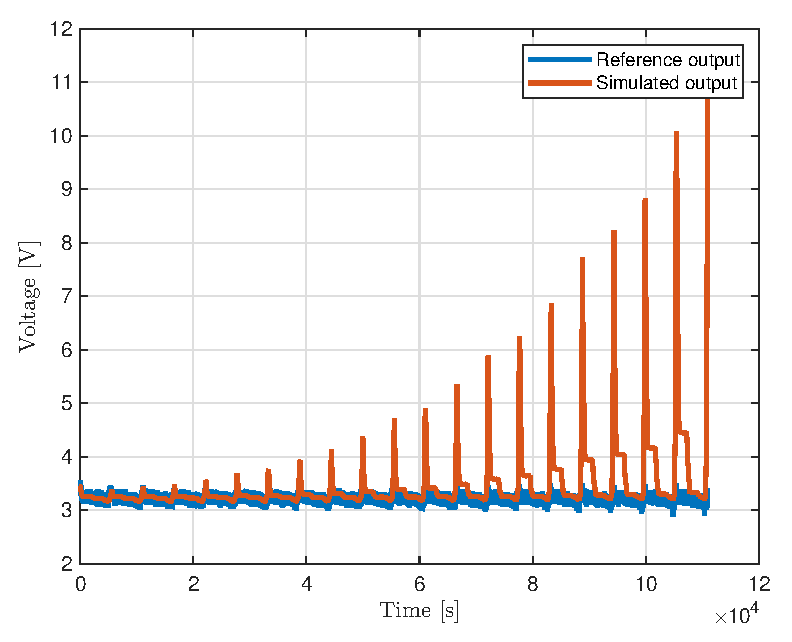
\includegraphics[width=\textwidth]{figures/9/validation-U.eps}
    \caption{Terminal voltage $\Ubat$.}
    \label{fig:9-validation-U}
    \end{subfigure}
    
    \caption{Comparison of reference and simulated waveforms.}
    \label{fig:9-validation}
\end{figure}

The dual EKF architecture was implemented regardless of the lack of information. Best results achieved using covariance matrices $\mathbf{R}_{\text{SoH}} = 1$, $\mathbf{R}_{\text{SoC}} = 0.05$, $\mathbf{Q}_{\text{SoH}} = diag(10^{-6}, 10^{-6}, 3\cdot 10^{-2})$ and $\mathbf{Q}_{\text{SoC}} = diag(10^{-8}, 10^{-10})$ are shown in Fig. \ref{fig:9-soc}. Both EKFs track the reference SoC with RMSE of 3.0 \%  over the whole experiment. The cell capacity $C$ estimated by SoH-EKF is shown in Fig. \ref{fig:9-capacity}. There is some non-negligible error (a 0.5 Ah bias) caused most probably by the mismatch of models used to generate reference data and to design the EKF. Nevertheless one can see the theoretical strenght of the dual EKF architecture for SoH estimation since the estimate capacity decreases with the same gradient as the reference.

\begin{figure}[hbp]
    \centering
\begin{subfigure}{0.49\textwidth}
    \centering
    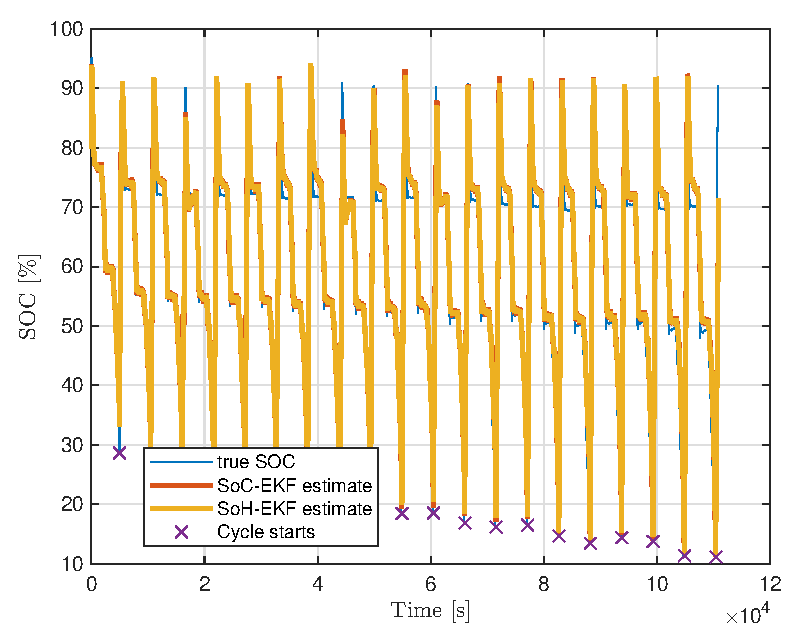
\includegraphics[width=\textwidth]{figures/9/soc-estimate.eps}
    \caption{SoC For the whole experiment.}
    \label{fig:9-soc-estimate}
    \end{subfigure}
    \hfill
    \begin{subfigure}{0.49\textwidth}
    \centering
    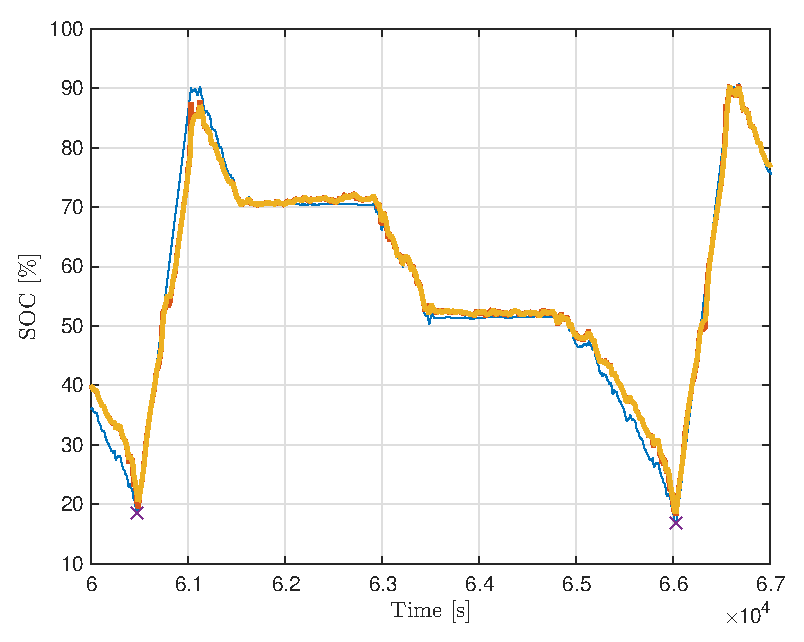
\includegraphics[width=\textwidth]{figures/9/soc-estimate-detail.eps}
    \caption{Detail of a single discharge-charge cycle.}
    \label{fig:9-soc-estimate-detail}
    \end{subfigure}
    
    \caption{SoC estimates given by the dual EKF architecture.}
    \label{fig:9-soc}
\end{figure}
 

\begin{figure}
    \centering
    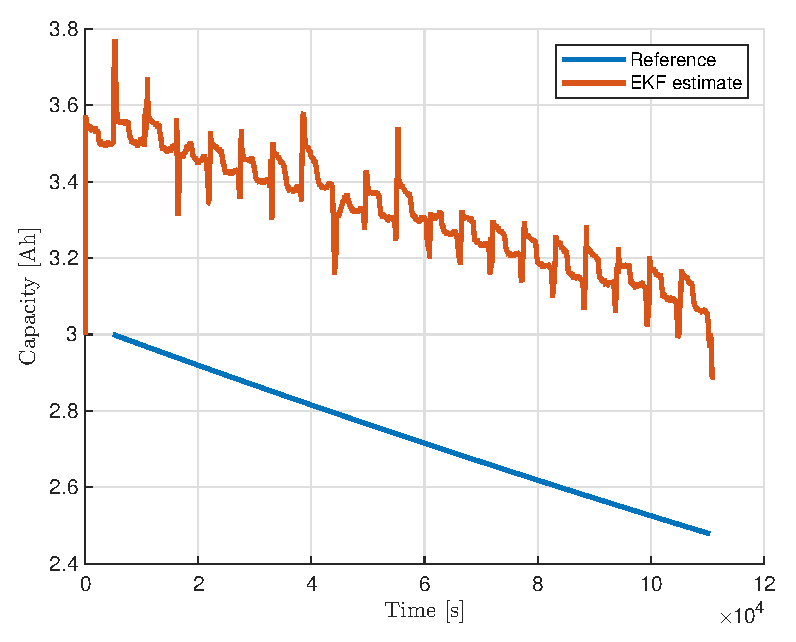
\includegraphics{figures/9/capacity-estimate.eps}
    \caption{Estimated and reference battery capacity}
    \label{fig:9-capacity}
\end{figure}


\chapter{Week 10 -- Online Parameter Estimation}


\section{Abstract}
This report presents an implementation of two methods for online estimation of battery model parameters. Recursive Least Squares (RLS) take a discrete-time transfer function and search for values of its coefficients. An Extended Kalman Filter (EKF) on the other hand considers the system in the state-space augmented by auxiliary states representing the -- possibly time-varying -- system parameters and estimates those. Both methods were derived for the battery equivalent circuit model with a single RC element and tested using a recording of a dynamic discharge profile.


\section{Recursive Least Squares}
\label{sec:10-rls}

For simplicity, consider the RLS algorithm for a simple ARX model, i.e. a general discrete-time transfer function in the time-domain delay operator $d$
\begin{equation}
    G(d) = \frac{Y(d)}{U(d)} = \frac{b_0 + b_1d + \dots + b_{n_b}d^{n_b}}{1 + a_1d + \dots + a_{n_a}d^{n_a}} = \frac{\sum_{i=0}^{n_b} b_i d^i}{\sum_{i=0}^{n_a} a_i d^i},
\end{equation}
usually normalized to unity $a_0$, i.e. the coefficient belonging to $y(k)$ in the corresponding difference equation
\begin{equation}
    y(k) + \sum_{i=1}^{n_a} a_i y(k-i) = \sum_{i=0}^{n_b} b_i u(k-i) + e(k)
    \label{eq:10-difference}
\end{equation}
relating past samples of the input $u$ and output $y$ up to the discrete time $k$. The variable $e(k)$ encapsulates stochastic phenomena such as noise, as well as unmodelled system dynamics.

The most recent output $y(k)$ can be predicted from \eqref{eq:10-difference} using past inputs and outputs and system parameters $\theta$ as
\begin{equation}
        \hat{y}(k) = - \sum_{i=1}^{n_a} a_i y(k-i) + \sum_{i=0}^{n_b} b_i u(k-i) ,
\end{equation}
that can be seen as a dot product
\begin{equation}
        \hat{y}(k) = \varphi^T(k) \theta(k)
        \label{eq:10-pred}
\end{equation}
of the regressor vector 
\begin{equation}
    \varphi(k) = \begin{bmatrix} -y(k-1) &-y(k-2) &\dots & -y(k-n_a) & u(k) & u(k-1) &\dots& u(k-n_b) \end{bmatrix}^T
\end{equation}
containing past inputs and outputs and the vector of parameters
\begin{equation}
    \theta(k) = \begin{bmatrix} a_1 & a_2 & \dots & a_{n_a} & b_0 & b_1 & \dots & b_{n_b} \end{bmatrix}^T.
\end{equation}

At each iteration $k$ of the RLS algorithm, the actual measured output $y(k)$ is compared with the prediction $\hat{y}(k)$ from \eqref{eq:10-pred} to find an error $e(k)$. Then the Kalman gain $K$ is calculated using the current estimate covariance matrix $\mathbf{P}$ and finally both the estimated system parameters $\hat{\theta}$ as well as the covariance matrix $\mathbf{P}$ are updated using $K$ and $e$. The algorithm can be extended by a real forgetting factor $\lambda \in \left[0, 1\right]$ used to artificially inflate the covariance matrix $\mathbf{P}$ to facilitate tracking of time-varying parameters.

The algorithm can be generalized and applied far beyond the limitation of linear ARX model. To use the RLS algorithm for any general problem, one needs to
\begin{enumerate}
    \item express the prediction task using an equation linear-in-parameters ,
    \item determine what expressions are to be estimated and belong to the parameter vector $\theta$
    \item determine what expressions are known  and belong to the regressor $\varphi$,
    \item find the (generally non-linear) mapping between parameters $\theta$ and physically meaningful parameters useful to the application.
\end{enumerate}

\subsection{RLS for battery parameters}

The continuous-time 1 RC equivalent circuit model reads
\begin{equation}
    \Ubat = \OCV - i \,R_0 - \underbrace{i \frac{R_1}{C_1  \,R_1\,  s+1}}_{U_1},
    \label{eq:10-ecm}
\end{equation}
where $i$ is the flowing current, $\Ubat$ is the measured terminal voltage, $\OCV$ is the cell's open-circuit voltage, $R_j$, $C_j$ are parameters of the model and $s$ is the Laplace transform operator. By relabeling $E = \Ubat - \OCV$, \eqref{eq:10-ecm} can be rewritten as a transfer function 
\begin{equation}
    G_\text{cont}(s) = -R_0 -\frac{R_1 }{C_1 \,R_1 \,s+1}
    \label{eq:10-tf}
\end{equation}
from the flowing current $i$ to the voltage drop $E$. The Tustin (bilinear) discretization of $G_\text{cont}(d)$ with step $T$ gives
\begin{equation}
    G(d) = \frac{{\left(R_0 \,T+R_1 \,T-2\,C_1 \,R_0 \,R_1 \right)}\,d+R_0 \,T+R_1 \,T+2\,C_1 \,R_0 \,R_1 }{{\left(2\,C_1 \,R_1 -T\right)}\,d-T-2\,C_1 \,R_1 }.
    \label{eq:10-G}
\end{equation}
Coparing \eqref{eq:10-G} to a general first-order discrete-time transfer function
\begin{equation}
    \frac{b_1 d + b_0}{a_1 d + 1}
\end{equation}
yields substitutions
\begin{align}
a_1 &=\frac{T-2\,C_1 \,R_1 }{T+2\,C_1 \,R_1 },\\
\label{eq:10-a1}
b_1 &=-\frac{R_0 \,T+R_1 \,T-2\,C_1 \,R_0 \,R_1 }{T+2\,C_1 \,R_1 },\\
b_0 &=-\frac{R_0 \,T+R_1 \,T+2\,C_1 \,R_0 \,R_1 }{T+2\,C_1 \,R_1 }.
\label{eq:10-b0}
\end{align}

Using the discretized transfer function $G(d)$, \eqref{eq:10-ecm} can be rewritten in several steps
\begin{align}
    \Ubat - \OCV &= i G(d), \\
    (\Ubat - \OCV)(a_1 d + 1) &=  i (b_1 d + b_0), \\
    \Ubat + \Ubat a_1 d - \OCV(a_1 d + 1) &=  i (b_1 d + b_0), \\
     \Ubat &= \OCV (a_1 d + 1) - \Ubat a_1 d + i (b_1 d + b_0).
     \label{eq:10-last}
\end{align}
Finally, assuming that the $\Delta \OCV$ is negligible on each sampling interval and therefore $\OCV(k) \approx \OCV(k-1)$, \eqref{eq:10-last} can be converted from the $d$-operator domain to index shifts
\begin{equation}
    \Ubat(k) = (a_1 + 1) \OCV - a_1 \Ubat(k-1) + b_0 i(k) + b_1 i(k-1).
    \label{eq:10-final}
\end{equation}
Equivalently in the short vector notation
\begin{equation}
    \Ubat(k) = \varphi^T(k) \theta,
\end{equation}
where
\begin{align}
    \theta &= \begin{bmatrix} (a_1 + 1) \OCV & a_1 & b_0 & b_1\end{bmatrix}^T, \label{eq:10-theta} \\ 
    \varphi(k) &= \begin{bmatrix} 1 & -\Ubat(k-1) & i(k) & i(k-1)\end{bmatrix}^T.
    \label{eq:10-varphi}
\end{align}

The problem at hand was successfully described using an equation \eqref{eq:10-final} that is linear in parameters $\theta$ and hence can be subject to RLS. Equations \eqref{eq:10-theta} and \eqref{eq:10-varphi} describe the role of individual variables ($\theta$ are estimated) and
equations \eqref{eq:10-a1} through \eqref{eq:10-b0} describe the nonlinear mappings from physically meaningful battery parameters to elements of $\theta$ with the inverse mapping given by
\begin{align}
R_0 &= \frac{b_0 -b_1 }{a_1 -1},\\
R_1 &= \frac{2\,{\left(b_1 -a_1 \,b_0 \right)}}{{a_1 }^2 -1}, \\
C_1 &= -\frac{T\,{a_1 }^2 -2\,T\,a_1 +T}{4\,{\left(b_1 -a_1 \,b_0 \right)}}.
\end{align}

Performance of the estimation algorithm is presented in Section \ref{sec:10-results}.

\section{Extended Kalman Filter}
\label{sec:10-ekf}

The EKF was discussed multiple times in previous reports, mainly as a great tool for SoC estimation. This time, it is used to estimate states of a state-space model augmented with model parameters. 
The 1 RC ECM from \eqref{eq:10-ecm} can be rewritten as a state-space
\begin{align}
    \dot{U_1} = - \frac{1}{R_1 C_1} U_1 + \frac{1}{C_1} i \\
    \Ubat = \OCV - i R_0 - U_1
    \label{eq:10-ss}
\end{align}
with input $i$, output $\Ubat$ and state $U_1$ (the polarization voltage). To estimate some model parameter $M$, it must be added to the list of system states. Without any apriori knowledge of parameter evolution, $\dot{M} = 0$ is assumed such that the parameter evolution is driven only by a random walk of the process noise.
Two distinct cell state-space representations based on the 1 RC equivalent circuit model were implemented and tested -- the reference model "Hongwen" with six states from \cite{hongwen} and my own manually derived model "Michal" with five states. Both models have the flowing current $i$ as input $u$ and the terminal voltage $\Ubat$ as output $y$.

\subsection{Hongwen model}
\label{sec:10-ekf-hongwen}
The Hongwen model considers six states
\begin{equation}
    x = \begin{bmatrix}
        \OCV & \Ubat & U_1  & \frac{1}{C_1} & \frac{1}{R_1} & R_0
    \end{bmatrix}^T
\end{equation}
with state equations
\begin{equation}
\begin{aligned}
    \dot{x_1} &= 0, \\
    \dot{x_2} &= x_1 x_4 x_5 - x_2x_4x_5 - (x_4 x_5 x_6 + x_4)u - x_6 \dot{u}, \\
    \dot{x_3} &= x_4 u - x_3 x_4 x_5, \\
    \dot{x_4} &= 0, \\
    \dot{x_5} &= 0, \\
    \dot{x_6} &= 0. \\
\end{aligned}
\end{equation}
This model includes the terminal voltage $\Ubat$ as state $x_2$, making the output equation trivial
\begin{equation}
    y = x_2.
\end{equation}
This model is quite complex and requires a non-standard addition of $\dot{u}$ (the derivative of input) that may introduce complications of its own.

\subsection{Michal model}
\label{sec:10-ekf-michal}
The Michal model eliminates the terminal voltage $\Ubat$ and considers only five states
\begin{equation}
    x = \begin{bmatrix}
        \OCV & U_1  & \frac{1}{C_1} & \frac{1}{R_1} & R_0,
    \end{bmatrix}^T
\end{equation}
with state equations
\begin{equation}
\begin{aligned}
    \dot{x_1} &= 0, \\
    \dot{x_2} &= x_3 u - x_2 x_3 x_4, \\
    \dot{x_3} &= 0, \\
    \dot{x_4} &= 0, \\
    \dot{x_5} &= 0 \\
\end{aligned}
\end{equation}
and a non-linear output equation
\begin{equation}
    y = x_1 - x_2 - u x_5.
\end{equation}
This model has fewer states, does not require the numeric differentiation of input $u$ and is generally much simpler than the Hongwen model. Results of online parameter estimation with both models are presented in Section \ref{sec:10-results}.

\clearpage
\section{Estimation results}
\label{sec:10-results}

All three methods (RLS estimation from Section \ref{sec:10-rls}, EKF for Hongwen model from Section \ref{sec:10-ekf-hongwen} and EKF for Michal model from \ref{sec:10-ekf-michal}) were compared using waveforms from a dynamic discharge profile. The achieved prediction error is shown in Fig. \ref{fig:10-pred}; Fig. \ref{fig:10-voltages} shows predictions throughout several DDP cycles whereas Fig. \ref{fig:10-pred-error} focuses on one DDP period. Low prediction error less than 10 mV confirms good convergence of model parameters to the behavior of the actual battery, although there is certainly some room for improvement (e.g. by introducing a second RC element).

\begin{figure}[hbp]
    \centering
\begin{subfigure}{0.49\textwidth}
    \centering
    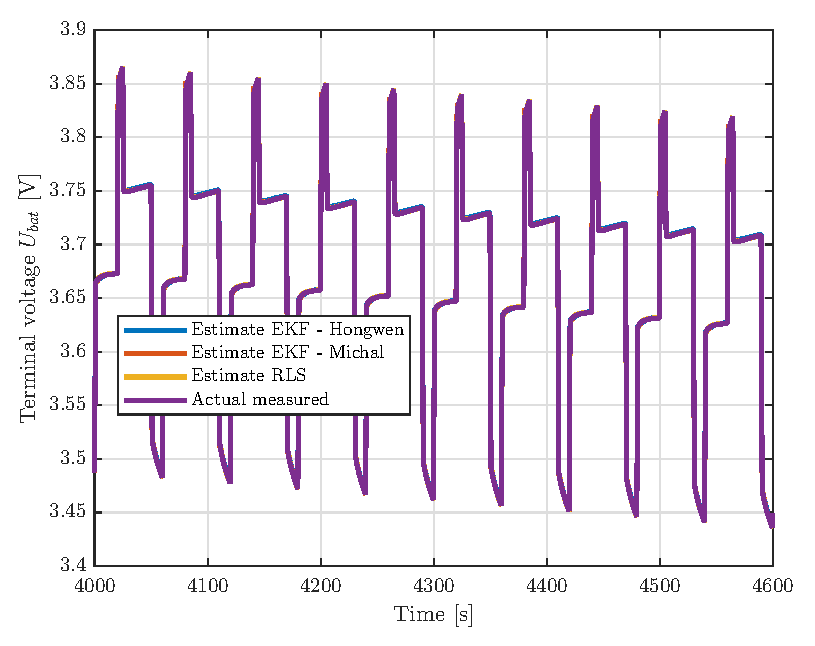
\includegraphics[width=\textwidth]{figures/10/voltages.eps}
    \caption{Over several DDP cycles.}
    \label{fig:10-voltages}
    \end{subfigure}
    \hfill
    \begin{subfigure}{0.49\textwidth}
    \centering
    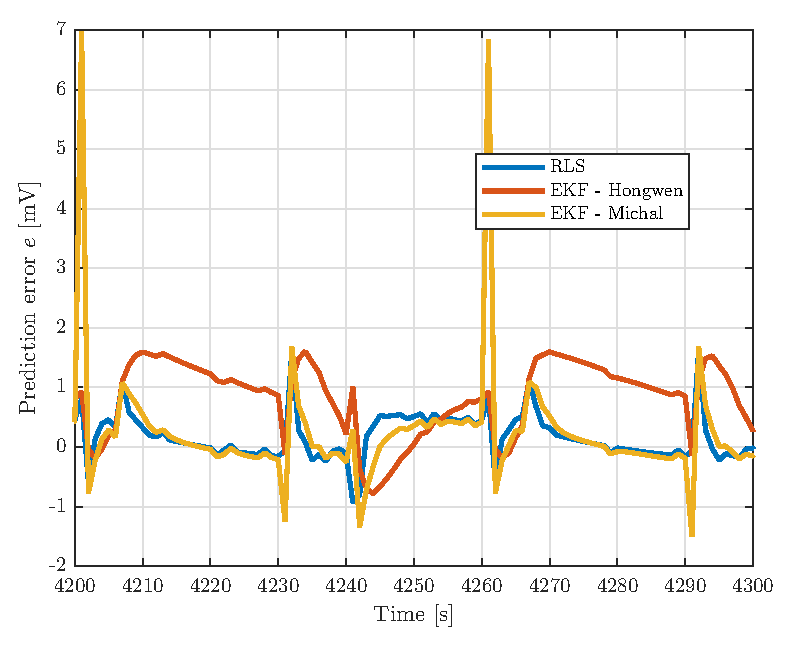
\includegraphics[width=\textwidth]{figures/10/voltages-pred-error.eps}
    \caption{Detail of one DDP period.}
    \label{fig:10-pred-error}
    \end{subfigure}
    
    \caption{Comparison of terminal voltages predicted by individual algorithms.}
    \label{fig:10-pred}
\end{figure}




\begin{figure}[hbp]
    \centering
\begin{subfigure}{0.49\textwidth}
    \centering
    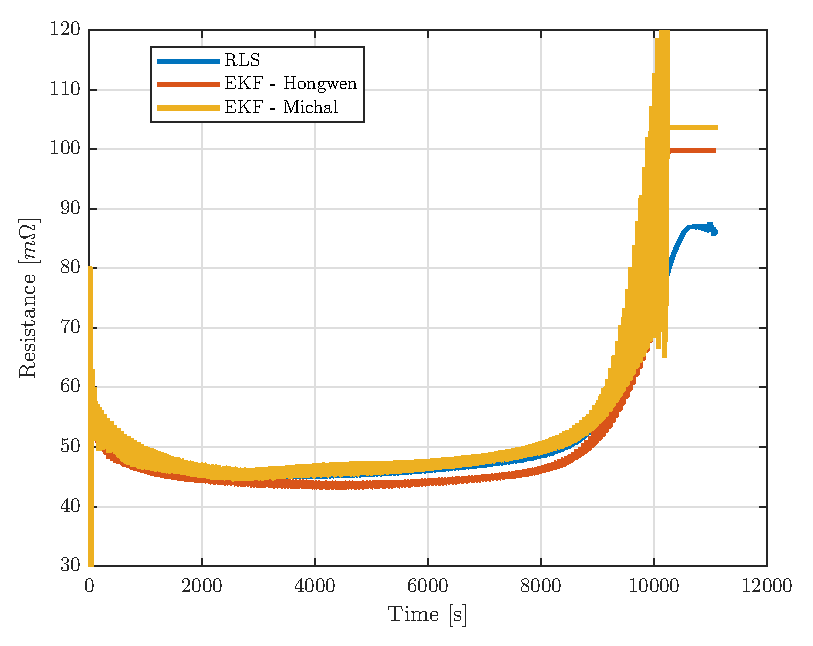
\includegraphics[width=\textwidth]{figures/10/est-R0.eps}
    \caption{Estimates of internal impedance $R_0$.}
    \label{fig:10-R0}
    \end{subfigure}
    \hfill
    \begin{subfigure}{0.49\textwidth}
    \centering
    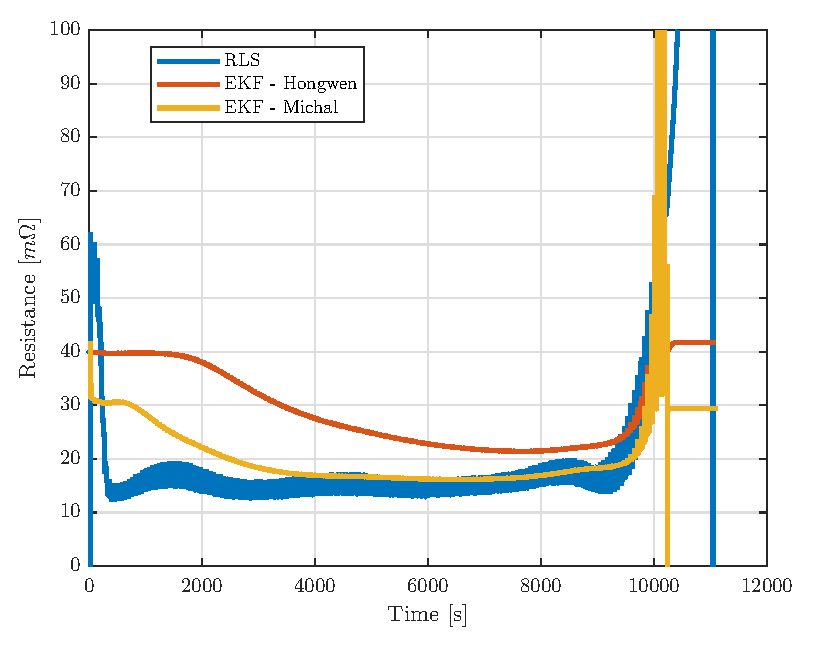
\includegraphics[width=\textwidth]{figures/10/est-R1.eps}
    \caption{Estimates of RC element resistance $R_1$.}
    \label{fig:10-R1}
    \end{subfigure}
    
    \caption{Estimates of resistive ECM parameters.}
    \label{fig:10-R}
\end{figure}

Estimates of both components of the ohmic (real) impedance $R_0$ and $R_1$ are shown in Fig. \ref{fig:10-R0} and Fig. \ref{fig:10-R1}, respectively. Estimates of $R_0$ yielded by various algorithms are quite similar and they demonstrate the expected (approximately) flat plateau roughly in the range of 80 \% to 20 \% of SoC with growing value towards extremes. On the other hand, estimates of $R_1$ shown in Fig. \ref{fig:10-R1} did not converge as satisfactorily with a significant discrepancy between both EKFs.

The estimated capacitance of the RC element shown in Fig. \ref{fig:10-C1} can be used to demonstrate an important difference between the RLS- and EKF-based parameter estimation. The EKF method allows the user to directly specify variance for individual physically meaningful parameters (albeit possibly inverted, such as $C_1^{-1}$). In contrast, the RLS works in terms of some artificial parameters $b_i$ and $a_i$, whose dependence on physically meaningful parameters is non-linear even for a 1 RC ECM and becomes increasingly more entangled with the growing number of parameters. Therefore, it is possible to get a smooth waveform for some given parameter (here $C_1$) with the EKF simply by reducing the parameter's variance. When estimating using RLS on the other hand, such fine control is very hard to do and the resulting estimate tends to be more noisy. A similar phenomenon can be observed in Fig. \ref{fig:10-R1}.

\begin{figure}[t]
\centering
\begin{minipage}{0.49\textwidth}
    \centering
    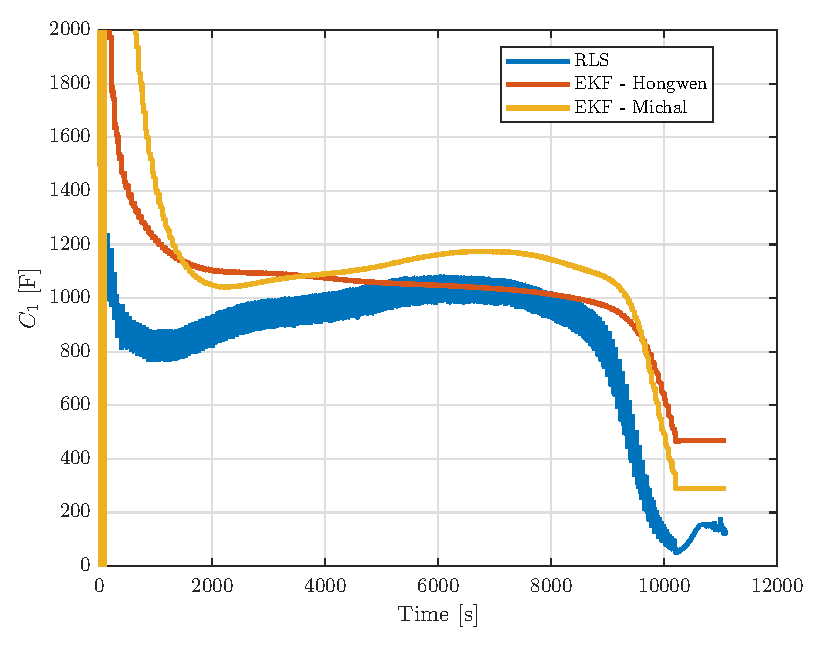
\includegraphics[width=\textwidth]{figures/10/est-C.eps}
    \caption{Estimates of RC element capacitance $C_1$.}
    \label{fig:10-C1}
\end{minipage}
\hfill
\begin{minipage}{0.49\textwidth}
    \centering
    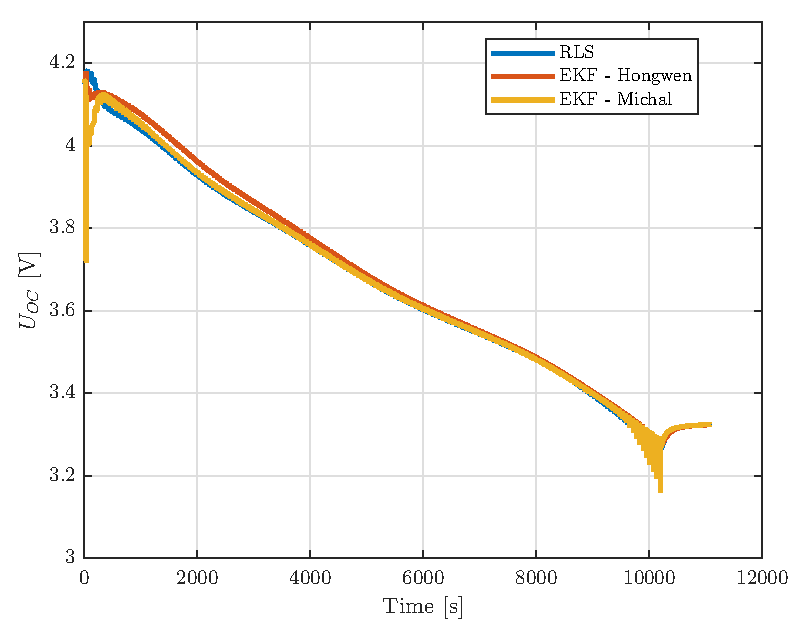
\includegraphics[width=\textwidth]{figures/10/est-OCV.eps}
    \caption{Estimates of the open circuit voltage $\OCV$.}
    \label{fig:10-OCV}
\end{minipage}
\end{figure}

All three methods estimate the $\OCV$ (shown in Fig. \ref{fig:10-OCV}) similarly well. The main difference from the implementation point of view is that the EKF method was far simpler to set up and debug owing to the tight bound of individual states to underlying physics. In contrast, the RLS method uses artificial (physically meaningless) parameters whose values must be post-processed to obtain any physically useful information. Typos such as an incorrect sign in some of the RLS expressions may cause a lot of headaches. Nevertheless, it is computationally less demanding than the EKF estimation and the forgetting factor $\lambda$ allows an intuitive configuration of the steady-state covariance matrix.

It is still unknown to me why the authors of \cite{hongwen} decided to use an unnecessarily complicated state space model for the parameter estimation task. Despite my best efforts in hyperparameter tuning (especially tuning the process noise covariance matrices $Q$), the simpler state-space model Michal achieved more credible results (closer matching the RLS estimates that I see as the best available reference in the absence of some ground truth parameter values) while being easier to debug and implement.


\chapter{Week 12 -- Data-Driven Methods}

\section{Abstract}
This report presents results of an experiment with data-driven methods and their use in battery modelling and prediction tasks. Using a dataset of 380 charging and discharging cycles from accelerated cell aging, a Random Forest regressor is trained to predict the remaining capacity of the cell (essentially predicting the SOH-C) using only a few pieces of information (features) from the full charging cycle.

\section{Familiarization with the environment}

In contrast to previous lab reports relying heavily on Matlab live scripts, this one was prepared using python in the Jupyer notebook environment. All tasks are performed on a dataset from the University of Michigan\footnote{available at \url{https://deepblue.lib.umich.edu/data/downloads/gq67jr501}}. It contains measurements such as cell voltage, current or temperature from 380 full battery cycles periodically sampled every 10 seconds. Since the task only deals with charging half-cycles, all time instants with current $i < \SI{0}{\ampere}$ are removed from the working dataset.

Most of the processing was done using the python library \texttt{pandas}. It provides means of loading the dataset using \texttt{pd.read\_csv}, accessing individual signals using \texttt{dataset[signal\_name]} and performing logical indexing (slicing) by \texttt{dataset[boolean\_mask]}. This is especially useful for operations such as extracting a particular full cycle or detecting discharging instants. Additionally, \texttt{matplotlib.pyplot} was used for visualization of signals.

The learning part of this lab was performed using the popular python package \texttt{scikit-learn}. It provides interface to many machine learning constructs such as metrics (loss functions, e.g. \texttt{mean\_squared\_error}), utilities such as \texttt{train\_test\_split} for simple creation of evaluation datasets for cross-validation, or the actual trainable models, such as the ensemble model \texttt{RandomForestRegressor} used in this task. 

\begin{figure}
\centering
\begin{minipage}{0.49\textwidth}
    \centering
    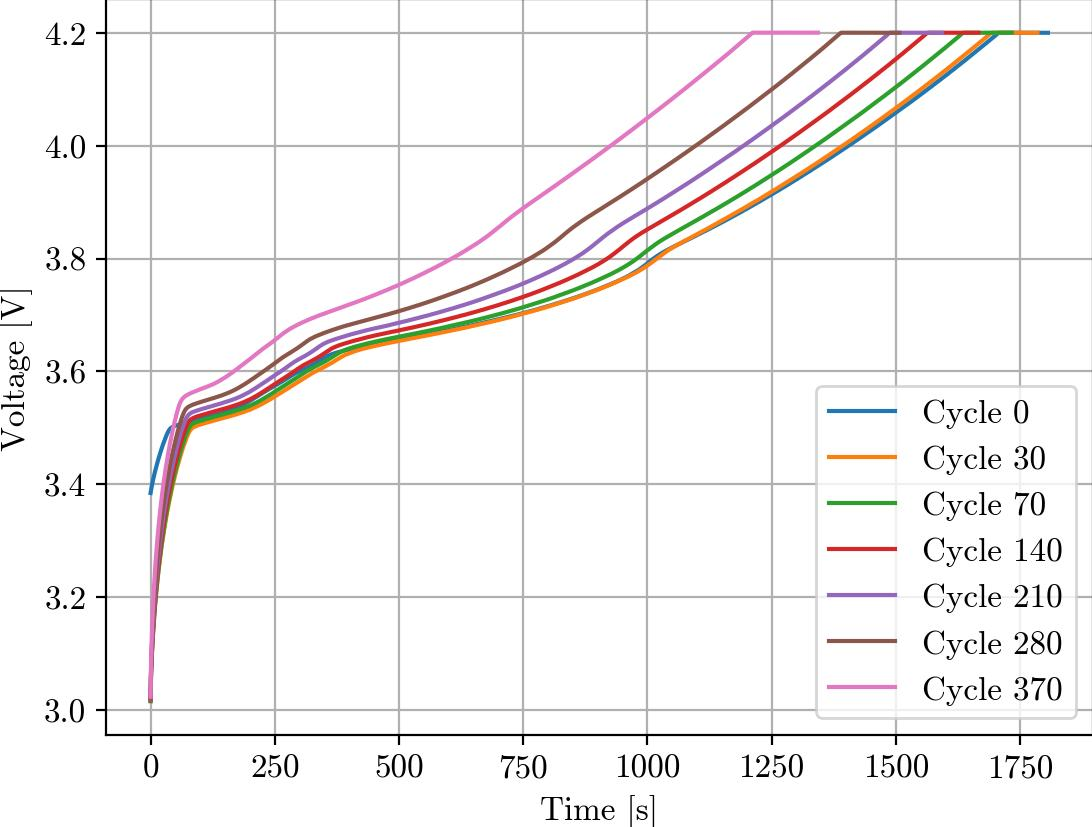
\includegraphics[width=\linewidth]{figures/12/voltages.jpg}
    \caption{Voltages during several full battery cycles.}
    \label{fig:12-voltages}
\end{minipage}
\hfill
\begin{minipage}{0.49\textwidth}
    \centering
    \includegraphics[width=\linewidth]{figures/12/currents.jpg}
    \caption{Currents during several full battery cycles.}
    \label{fig:12-currents}
\end{minipage}
\end{figure}

\section{Training the regressor}

To verify that the provided dataset can be used for the training of an SOH-C predictor, one can plot and analyze measurements from several cycles. Fig. \ref{fig:12-voltages} through \ref{fig:12-capacities} show the recorded cell voltage, flowing current and capacity, respectively. The charging mode is clearly CC-CV with current limit of 1000 mA and target voltage of 4.2 V. It is apparent from all figures/12 that with a growing number of elapsed cycles, the cell ages and loses capacity, making subsequent cycles shorter (the voltage in Fig. \ref{fig:12-voltages} rises faster and the current in \ref{fig:12-currents} drops earlier). 
Additionally, the total capacity gradually decreases, as shown in Fig. \ref{fig:12-aging}. There are several outlier cycles that were interrupted early for unspecified reasons.

Out of the total of 380 recorded cycles, 19 were randomly selected for final testing. The rest was divided into the training and validation dataset according to the 80:20 Pareto rule. Instead of using all collected samples (roughly 2000 of them per signal per cycle) as inputs to the machine learning algorithm, information from each cycle is condensed into a small vector of features. The Random Forrest is an ensemble algorithm for supervised learning that separately trains many decision trees on subsets of the training data and then combines (e.g. averages) their outputs when asked to predict the output for previously unseen data. In this task, the number of trees in the forest (an algorithm hyperparameter) was chosen as 100.

\begin{figure}
\centering
\begin{minipage}{0.49\textwidth}
    \centering
    \includegraphics[width=\linewidth]{figures/12/capacities.jpg}
    \caption{Cell capacity during several full battery cycles.}
    \label{fig:12-capacities}
\end{minipage}
\hfill
\begin{minipage}{0.49\textwidth}
    \centering
    \includegraphics[width=\linewidth]{figures/12/aging.jpg}
    \caption{The loss of total cell capacity due to aging.}
    \label{fig:12-aging}
\end{minipage}
\end{figure}

\subsection{Selection of features}

The best performance (the lowest error on the test set) was achieved using the features listed in Table \ref{tab:12-importance} in the decreasing order of mean importance. Said simply\footnote{More detailed explanation of the feature importance can be found at \url{https://medium.com/the-artificial-impostor/feature-importance-measures-for-tree-models-part-i-47f187c1a2c3} and in resources linked there.}, the \textit{Mean Decrease in Impurity (MDI)} used by \texttt{scikit} measures the importance of a feature as the number of decision nodes that branch paths based on said feature weighted by the probability of reaching said nodes. 
High feature importance means that many decision tree nodes are branching the path based on said feature and that they reside in busy subtrees of the whole tree hit by many input samples.
On the other hand, negligible feature importance shows that the tree did not need to incorporate said feature into its decision nodes during training. Since this metric is calculated for each tree separately, the third column of Table \ref{tab:12-importance} shows the standard deviation of importances across the whole forest. Note that many of these standard deviations are quite significant, hinting that indeed each tree puts emphasis on entirely different features.

\begin{table}[]
    \centering
    \begin{tabular}{c|c|c}
    Feature name & Mean importance & Standard deviation of importance \\ \hline
Temperature Delta & 0.4250 & 0.3142 \\
Number of Samples & 0.3646 & 0.2996 \\
Total Charge   & 0.1022 & 0.1987 \\
Average Current & 0.0411 & 0.1223 \\
Maximal V      & 0.0360 & 0.1129 \\
Current Standard Deviation & 0.0216 & 0.0830 \\
Average Temperature & 0.0048 & 0.0329 \\
Minimal V      & 0.0047 & 0.0333 \\
    \end{tabular}
    \caption{Importance of individual features for individual trees in the ensemble model}
    \label{tab:12-importance}
\end{table}

The presence of the number of samples collected during the charging cycle among the most important features is expected, as it indirectly expresses the duration of charging half-cycle and that is significantly influenced by the cell's capacity when using CC-CV scheme, as shown e.g. in Fig. \ref{fig:12-currents}. However what is not expected at all is the high importance of the temperature delta. In order to explain it, measurements of the cell's internal resistance available in the dataset have to be used. The evolution of the real part of cell's impedance as a function of the available capacity over the course of the experiment is shown in Fig. \ref{fig:12-R}. The ohmic resistance clearly grows (yet again proving that the dataset indeed describes a noticeably aging cell, in this case with respect to SOH-R), causing increased losses due to constant charging current, eventually resulting in greater temperature delta.

Some features on the other hand were identified by the algorithm as mostly irrelevant, e.g. the minimal and maximal voltage. This can be explained intuitively as well - all charging half-cycles end at 4.2 V (giving no useful information about the cell capacity) and the starting voltage is subject to slight unpredictable variation caused by transition from one cycle to the next.

\begin{figure}
    \centering
    \includegraphics[width=0.5\linewidth]{figures/12/R.jpg}
    \caption{Real part of the cell impedance during ageing}
    \label{fig:12-R}
\end{figure}

\subsection{Evaluation of the Regressor}

The model's performance after training was evaluated using the test set. True cell capacities and the corresponding model predictions are shown in Fig. \ref{fig:12-pred}. The histogram of prediction errors shown in Fig. \ref{fig:12-pred-error-hist} suggests that the model tends to underestimate the true capacity slightly (by less than 15 mAh) with the exception of two outliers with grater prediction error.
The algorithm's performance was assessed using several metrics listed in Table \ref{tab:12-test-error}. Their values are derived from the prediction error expressed in Ah, i.e. the greatest single prediction error was 22.9 mAh and the average prediction error was 6.93 mAh.

\begin{table}[]
    \centering
    \begin{tabular}{c|c}
        Error metric & Magnitude \\\hline
        Maximal error                  & 2.29e-02 \\
        Mean Absolute Deviation (MAD)  & 6.93e-03 \\
        Mean squared error (MSE)       & 8.35e-05 \\
    \end{tabular}
    \caption{Prediction error achieved on the test set}
    \label{tab:12-test-error}
\end{table}




\begin{figure}
\centering
\begin{minipage}{0.49\textwidth}
    \centering
    \includegraphics[width=\linewidth]{figures/12/test.jpg}
    \caption{Regressor performance on the test set.}
    \label{fig:12-pred}
\end{minipage}
\hfill
\begin{minipage}{0.49\textwidth}
    \centering
    \includegraphics[width=\linewidth]{figures/12/pred-error-hist.jpg}
    \caption{Capacity prediction error on the test set.}
    \label{fig:12-pred-error-hist}
\end{minipage}
\end{figure}





\chapter{Week 13 -- Overcurrent Protection For A Modular System}

\section{Abstract}
This report presents results of tuning a high-level supervisory algorithm that calculates a system-level current limit respecting the current limitation of individual modules connected in parallel. Different initial conditions of individual modules are assumed for generality. Two solutions are considered -- a feedforward approach based on the closed-form expression for current upper and lower bound using the provided voltage, current and internal resistance of each module, and a feedback solution using a modified PID controller regulating the module current towards the module current limit. 


\section{Problem statement}



\begin{figure}[b]
\centering
\begin{minipage}{0.49\textwidth}
    \centering
    \includegraphics[width=\linewidth]{figures/13/ff-R.pdf}
    \caption{Estimates of the module internal impedance available to the algorithm.}
    \label{fig:13-R}
\end{minipage}
\hfill
\begin{minipage}{0.49\textwidth}
    \centering
    \includegraphics[width=\linewidth]{figures/13/ff-SoC.pdf}
    \caption{Module state of charge (SoC) during the simulation.}
    \label{fig:13-SoC}
\end{minipage}
\end{figure}

\begin{figure}[]
\centering
\begin{minipage}{0.49\textwidth}
    \centering
    \includegraphics[width=\linewidth]{figures/13/fb-IE.pdf}
    \caption{Equalizing current flowing from module 1 to module 2.}
    \label{fig:13-IE}
\end{minipage}
\hfill
\begin{minipage}{0.49\textwidth}
    \centering
    \includegraphics[width=\linewidth]{figures/13/ff-U.pdf}
    \caption{Module terminal voltages.}
    \label{fig:13-U}
\end{minipage}
\end{figure}

The given Simulink model contains a model of two battery modules connected in parallel, each consisting of a 1RC equivalent circuit model (ECM). Each module is given a different initial SoC, as shown in fig. \ref{fig:13-SoC} and also different parameters of the ECM, such as internal impedance $R_0$ shown in Fig. \ref{fig:13-R}. This alone results in some current asymmetry between both modules due to the flow of an equalizing current shown in Fig. \ref{fig:13-IE}. Since both modules are connected in parallel, their terminal voltages must be equal by definition. This is verified in Fig. \ref{fig:13-U}, showing maximal voltage deviation in the order of $10^{-4}$ V.

Each module is given a current limit of 50 A for both charging and discharging. During the experiment, some connected system (e.g. the motor controller of an EV) requests current for vehicle propulsion and the battery system must restrict the current flow to a safe system-wide limit such that neither of the modules is overloaded.

The task is complicated by the measurement noise that is gradually added to the quantities provided to the control algorithm. Furthermore, the estimate of module impedance is subject to significant disturbance, resulting in large variations of the estimate of $R_0$ available for the current limit calculation, as shown in Fig. \ref{fig:13-R}.

\section{Analytical solution}

The first solution utilized an algorithm based on a closed-form expression for the current limit. Measured module voltages, currents and impedances are used to calculate the equalizing current $I_E$. Then, considering the current divider formed by impedances $R_{0,1}$ and $R_{0,2}$, a set of inequalities for the upper bounds of the system current is constructed. The lowest bound is then used to prevent exceeding the current limit fo any module.

Results obtained by this algorithm are shown in Fig. \ref{fig:13-ff-system} and \ref{fig:13-ff-subsystem}. The algorithm has the potential to work very well when provided with correct information (as shown for $t<150$ s), where the current through the first module is saturated perfectly at the module current limit. Nevertheless, as soon as the estimate of $R_0$ becomes noisy or completely wrong, the inherently open-loop solution can't optimally deliver the requested current. This is illustrated for $t > 450$ s, when the system-wide current limit abruptly decreases due to the error of resistance estimates from Fig. \ref{fig:13-R}.

Due to this inherent limitation, the algorithm was not even completely implemented and yielded incorrect results when approaching the negative lower bound. The alternative feedback solution achieved much better performance; hence, it was not worthwhile to attempt to fix the feedforward algorithm. 

\begin{figure}
\centering
\begin{minipage}{0.49\textwidth}
    \centering
    \includegraphics[width=\linewidth]{figures/13/ff-system.pdf}
    \caption{System currents using the feedforward control algorithm.}
    \label{fig:13-ff-system}
\end{minipage}
\hfill
\begin{minipage}{0.49\textwidth}
    \centering
    \includegraphics[width=\linewidth]{figures/13/ff-subsystem.pdf}
    \caption{Subsystem currents using the feedforward algorithm.}
    \label{fig:13-ff-subsystem}
\end{minipage}
\end{figure}

\section{Feedback algorithm}

The feedback algorithm uses a modified PID controller to determine the system-wide current limit. First, since the module current limit is symmetric for charging and discharging, the maximum of absolute values of both module currents is taken to simplify calculations by considering only the positive branch. This maximal current is subtracted from the module current limit to get an error that is fed to the discrete-time PID controller with filtered derivative. The output of the PID controller was saturated at twice the module current limit -- that is the optimistic solution in case both modules are balanced and there is no equalizing current.

To further improve the behavior of the PID controller, the following trick was introduced -- the error is scaled down by a factor of 1000 when it is positive. This way, the current limit is quickly adjusted down to prevent stress to battery modules, while the growth of the current limit is very slow to ensure smooth waveform.

The performance of this algorithm is shown in Fig. \ref{fig:13-fb-system} and \ref{fig:13-fb-subsystem}. It is clear that the algorithm asymptotically delivers the maximal possible current whilst achieving overshoots of both low height as well as area, as shown in Fig. \ref{fig:13-fb-subsystem-detail} and \ref{fig:13-fb-subsystem-detail2}. Typical overshoot is less than 8 A in height and lasts for less than 400 ms.

\begin{figure}
\centering
\begin{minipage}{0.49\textwidth}
    \centering
    \includegraphics[width=\linewidth]{figures/13/fb-system.pdf}
    \caption{System current using the feedback control algorithm.}
    \label{fig:13-fb-system}
\end{minipage}
\hfill
\begin{minipage}{0.49\textwidth}
    \centering
    \includegraphics[width=\linewidth]{figures/13/fb-subsystem.pdf}
    \caption{Subsystem currents using the feedback algorithm.}
    \label{fig:13-fb-subsystem}
\end{minipage}
\end{figure}


\begin{figure}
\centering
\begin{minipage}{0.49\textwidth}
    \centering
    \includegraphics[width=\linewidth]{figures/13/fb-subsystem-detail.pdf}
    \caption{Overshoots of the module current limit}
    \label{fig:13-fb-subsystem-detail}
\end{minipage}
\hfill
\begin{minipage}{0.49\textwidth}
    \centering
    \includegraphics[width=\linewidth]{figures/13/fb-subsystem-detail2.pdf}
    \caption{Detail of one particular overshoot of the OCP limit.}
    \label{fig:13-fb-subsystem-detail2}
\end{minipage}
\end{figure}

Fig. \ref{fig:13-fb-system-detail} illustrates that a step of the requested system current from 0 to 120 A results in a decrease of the current limit from 94 A to 86 A. This was the worst case (greatest in magnitude) sudden change observed in the simulation outputs.

\begin{figure}
    \centering
    \includegraphics[width=0.5\linewidth]{figures/13/fb-system-detail.pdf}
    \caption{Response of the system-wide current limit to a step of requested current.}
    \label{fig:13-fb-system-detail}
\end{figure}

\section{Conclusions}

The achieved performance could be further improved by giving the algorithm access to the requested current. That way, the algorithm could identify time instants when the flow of current is saturated and only then activate the integrator to slowly increase the system-wide current limit. Without this information the algorithm has to slowly increase the current limit at all times in order to be able to quickly deliver the maximal possible current.



% VoMi uncomment this to learn the width of our page (for matlab to properly plot stuff)
%\showthe\textwidth % For single column documents
%\showthe\columnwidth % For multiple column documents

\chapter{Week 14 -- Offline SoH Estimation}

% The paper headers



% As a general rule, do not put math, special symbols or citations
% in the abstract or keywords.
\section{Abstract}
This report presents an implementation and results of two offline state of health evaluation methods. The assignment provided measured data from a single cell after 0, 12000 and 24000 cycles, namely the impedance data from Electrochemical Impedance Spectroscopy (EIS) and the voltage-capacity dependence for calculation of Differential Voltage (DV) and Incremental capacity (IC) curves. Visualized samples from individual experiments were compared both qualitatively and quantitatively.


\section{EIS}

\begin{figure}[hbp]
    \centering
\begin{subfigure}{0.49\textwidth}
    \centering
    \includegraphics[width=\textwidth]{figures/14/EIS-impedance-measured.pdf}
    \caption{Measured samples.}
    \label{fig:14-EIS-measured}
    \end{subfigure}
    \hfill
    \begin{subfigure}{0.49\textwidth}
    \centering
    \includegraphics[width=\textwidth]{figures/14/EIS-impedance-fit.pdf}
    \caption{Measured and fitted curves.}
    \label{fig:14-EIS-fit}
    \end{subfigure}
    
    \caption{Evolution of EIS curves as the cell under test ages.}
    \label{fig:14-EIS}
\end{figure}

All provided EIS data correspond to SoC of 60 \%. The data was preprocessed according to the standard method -- first remove samples with $\Im Z > 0$ (as the indictive character is more influenced by parasitic properties of wires and cell tabs rather than the battery itself) and then flip the sign of $\Im Z$ in the remaining samples to get a plot in the first quadrant. The remaining measured samples are shown in Fig. \ref{fig:14-EIS-measured}. There is a noticeable trend that the inflexion point moves right to higher real parts of the total impedance. It should be noted that the available data does not show a noticeable change in $R_0$ over the cell's lifetime. This indicates that the resistance of conductors stayed mostly unchanged, and rather only the electrochemical part was subject to degradation.

To fit the provided EIS curves, the parameterized impedance of a equivalent circuit proposed in \cite{fernandez} was calculated. It was composed a series interconnection of blocks
\begin{enumerate}
    \item real impedance $R_0$,
    \item $R_{SEI}$ in parallel to a constant phase element (CPE),
    \item $R_{ct}$ in series with semi-infinite Warburg, the whole branch in parallel to a CPE.
\end{enumerate}

\begin{table}[]
    \centering
    \begin{tabular}{c||c|c|c|c||c|c|c}
        Number of cycles & $R_0$ [m$\Omega$] & $R_{SEI}$ [m$\Omega$] & $R_{ct}$ [m$\Omega$] & $R_{W}$ [m$\Omega$] & CL [\%] & LLI [\%] & LAM [\%] \\ \hline \hline
        0 & 16.36 & 3.28 & 3.91 & 5.57 & 0.00 & 0.00 & 0.00 \\
        12000 & 16.71 & 3.93 & 6.19 & 5.98 & 2.13 & 40.82 & 7.38 \\
        24000 & 16.21 & 5.32 & 4.80 & 8.08 & -0.94 & 40.87 & 45.15 \\

    \end{tabular}
    \caption{Equivalent circuit parameters fitted from EIS measurements.}
    \label{tab:14-eis}
\end{table}

Fitted curves are shown in Fig. \ref{fig:14-EIS-fit} and parameters are important parameters are listed in Table \ref{tab:14-eis}. The last three columns additionally include the evaluated "growth in percentage" $G_{EIC}$ metric for individual degradation modes, namely conductivity loss (CL), Lithium loss inventory (LLI) and loss of active material (LAM). Analyzing the table more closely, due to the negligible variance of $R_0$, the conductivity loss is a very unlikely degradation mode. On the other hand the growth of SEI (Solid Electrolyte Interface) resistance $R_{SEI}$ and charge transfer resistance $R_{ct}$ hint at significant loss of Lithium inventory (LLI). Finally, the increasing Warburg resistance $R_W$ hints at gradual loss of active material (LAM) degradation mode.




\section{IC/DV Analysis}

A similar analysis can be performed using the time-domain data from a charging half-cycle -- ideally with low charging current to obtain pseudo OCV curves, but the assignment only provided CC-CV charging with 1.5 A of current. The measured relation between cell terminal voltage and the current capacity is shown in Fig. \ref{fig:14-QU} for three distinct charging half-cycles throughout the cell's lifetime. The first obvious observation is that as the cell ages, the total capacity decreases, hence the CC-CV charging ends earlier at lower capacity.

\begin{figure}
    \centering
    \includegraphics[width=0.5\textwidth]{figures/14/QU.pdf}
    \caption{Collected voltage-capacity data from three charging half-cycles.}
    \label{fig:14-QU}
\end{figure}

\begin{figure}[b]
\centering
\begin{minipage}{0.49\textwidth}
    \centering
    \includegraphics[width=\textwidth]{figures/14/IC.pdf}
    \caption{Evolution of Incremental capacity (IC) during cell's lifetime.}
    \label{fig:14-IC}
\end{minipage}
\hfill
\begin{minipage}{0.49\textwidth}
    \centering
    \includegraphics[width=\textwidth]{figures/14/DV.pdf}
    \caption{Evolution of Differential voltage (DV) during cell's lifetime.}
    \label{fig:14-DV}
\end{minipage}
\end{figure}

To facilitate the calculation of Incremental capacity and Differential Voltage curves, the data was preprocessed to suppress measurement noise using a Savitzky-Golay Filter of order 3 and frame length 501 samples. Subsequently duplicated neighbouring measurements resulting in division by zero were eliminated.
Both curves for all experiments are shown in Fig. \ref{fig:14-IC} and \ref{fig:14-DV}, respectively. Again, there are some clear differences between the reference curves corresponding to 0 cycles and curves corresponding to points later in the cell's life -- for example the DV curve in Fig. \ref{fig:14-DV} gets overall higher whilst the IC curve in \ref{fig:14-IC} overall moves down since as the total capacity decreases with cell's age, lower amount of charge is needed to increase the terminal voltage.

Using formulae from \cite{fernandez}, degradation mode indicators for CL, LLI and LAM listed in Table \ref{tab:14-icdv} were calculated. Obtained results roughly match the conclusion from EIS (see \ref{tab:14-eis}) -- the cell aged in a way that did not influence the resistance of conductors, whereas both LLI and LAM are noticeable.







\begin{table}[]
    \centering
    \begin{tabular}{c||c|c|c}
        Number of cycles & CL [\%] & LLI [\%] & LAM [\%] \\ \hline \hline
        0 & 0.00e+00 & 0.00 & 0.00 \\
        12000 & 2.72e-05 & 8.98 & 9.64 \\
        24000 & 1.53e-02 & 11.42 & 12.89 \\

    \end{tabular}
    \caption{Degradation modes identified using IC/DV curves.}
    \label{tab:14-icdv}
\end{table}





\IEEEpeerreviewmaketitle






\ifCLASSOPTIONcaptionsoff
  \newpage
\fi

\begin{thebibliography}{9}

    \bibitem{hongwen}
Hongwen He, et al.
\emph{"Online estimation of model parameters and state-of-charge of LiFePO4 batteries in electric vehicles"},
Applied Energy,
Volume 89, Issue 1,
2012,
https://doi.org/10.1016/j.apenergy.2011.08.005.
    
    \bibitem{fernandez}
    Carlos Pastor-Fernández et al.,
    \emph{"A Comparison between Electrochemical Impedance Spectroscopy and Incremental Capacity-Differential Voltage as Li-ion Diagnostic Techniques to Identify and Quantify the Effects of Degradation Modes within Battery Management Systems"},
    Journal of Power Sources,
    2017,
    https://doi.org/10.1016/j.jpowsour.2017.03.042,
    Available online at https://www.sciencedirect.com/science/article/pii/S0378775317303269

\end{thebibliography}


% that's all folks
\end{document}